\documentclass[sigconf]{acmart}
% 
% LaTeX template for visualizing the performance of
% optimization algorithms, that were run on the 
% bbob test suite of COCO. Any number of 
% algorithms should work with this template.

% include preamble:
%%%%%%%%%%%%%%%%%%%%%%%%%%%%%%%%%%%%%%%%%%%%%%%%%%%%%%%%%%%%%%%%%%%%%%%%%%%%%%%
% preamble for the BBOB ACM-compliant LaTeX templates                         %
%                                                                             %
% copyright 2009--2023 the BBOBies                                            %
% (under BSD licence, see https://github.com/numbbo/coco/blob/master/LICENSE) %
%%%%%%%%%%%%%%%%%%%%%%%%%%%%%%%%%%%%%%%%%%%%%%%%%%%%%%%%%%%%%%%%%%%%%%%%%%%%%%%

% to be updated from year to year:
\titlenote{Submission deadline: to be announced (likely late March/early April.}
\newcommand{\version}{2.6}


% Packages
\usepackage{booktabs} % For formal tables
\usepackage{graphicx}
\usepackage{rotating}
\usepackage{tabularx}
\usepackage{xspace}  % automatic white space after macros
\usepackage{xstring} % for string operations
\usepackage{wasysym} % Table legend with symbols input from post-processing
\usepackage{MnSymbol} % Table legend with symbols input from post-processing
\usepackage{float}
%\usepackage[dvipsnames]{xcolor}
%\usepackage[colorlinks=true, linkcolor=blue]{hyperref} % make COCO papers clickable
\usepackage{ifthen}
\usepackage{xcolor}



% define some COCO/dvipsnames colors because
% ACM style does not allow to use them directly
\definecolor{Gray}{gray}{0.6}
\definecolor{NavyBlue}{rgb}{0.0, 0.0, 0.5}
\definecolor{Magenta}{rgb}{1.0, 0.0, 1.0}
\definecolor{Black}{rgb}{0.0, 0.0, 0.0}
\definecolor{Green}{rgb}{0.0, 1.0, 0.0}
%\definecolor{NavyBlue}{HTML}{000080}
%\definecolor{Magenta}{HTML}{FF00FF}
%\definecolor{Orange}{HTML}{FFA500}
%\definecolor{CornflowerBlue}{HTML}{6495ED}
%\definecolor{YellowGreen}{HTML}{9ACD32}
%\definecolor{Gray}{HTML}{BEBEBE}
%\definecolor{Yellow}{HTML}{FFFF00}
%\definecolor{GreenYellow}{HTML}{ADFF2F}
%\definecolor{ForestGreen}{HTML}{228B22}
%\definecolor{Lavender}{HTML}{FFC0CB}
%\definecolor{SkyBlue}{HTML}{87CEEB}
%\definecolor{NavyBlue}{HTML}{000080}
%\definecolor{Goldenrod}{HTML}{DDF700}
%\definecolor{VioletRed}{HTML}{D02090}
%\definecolor{CornflowerBlue}{HTML}{6495ED}
%\definecolor{LimeGreen}{HTML}{32CD32}

% COCO LaTeX commands:
\newcommand{\includeperfprof}[1]{% include and annotate at the side
  \input{\bbobdatapath\algsfolder #1}%
  \includegraphics[height=0.24\textheight]{#1}%
  %\raisebox{.12\textheight}{
	%\parbox[b][.24\textheight]{.0868\textwidth}{\begin{scriptsize}
  %  \perfprofsidepanel % this is "\algaperfprof \vfill \algbperfprof \vfill" etc
  %\end{scriptsize}}
	%}
}
\newcommand{\rot}[2][2.5]{
  \hspace*{-3.5\baselineskip}%
  \begin{rotate}{90}\hspace{#1em}#2
  \end{rotate}}
\newcommand{\DIM}{\ensuremath{\mathrm{DIM}}}
\newcommand{\ERT}{\ensuremath{\mathrm{ERT}}}
\newcommand{\FEvals}{\ensuremath{\mathrm{FEvals}}}
\newcommand{\nruns}{\ensuremath{\mathrm{Nruns}}}
\newcommand{\Dfb}{\ensuremath{\Delta f_{\mathrm{best}}}}
\newcommand{\Df}{\ensuremath{\Delta f}}
\newcommand{\Dfg}{\ensuremath{\Delta \tau}}
\newcommand{\nbFEs}{\ensuremath{\mathrm{\#FEs}}}
\newcommand{\fopt}{\ensuremath{f_\mathrm{opt}}}
\newcommand{\ftarget}{\ensuremath{f_\mathrm{t}}}
\newcommand{\fgtarget}{\ensuremath{\tau_\mathrm{t}}}
\newcommand{\Itarget}{\ensuremath{I_\mathrm{target}}}
\newcommand{\CrE}{\ensuremath{\mathrm{CrE}}}
\newcommand{\change}[1]{{\color{red} #1}}
\newcommand{\TODO}[1]{{\color{orange} !!! #1 !!!}}
\newcommand{\bbob}{{\ttfamily bbob}\xspace}
\newcommand{\bbobnoisy}{{\ttfamily bbob-noisy}\xspace}
\newcommand{\bbobbiobj}{{\ttfamily bbob-biobj}\xspace}
\newcommand{\bbobls}{{\ttfamily bbob-largescale}\xspace}
\newcommand{\bbobmixint}{{\ttfamily bbob-mixint}\xspace}
\newcommand{\bbobcons}{{\ttfamily bbob-constrained}\xspace}
\newcommand{\DI}{\ensuremath{\Delta I_{\mathrm{HV}}^{\mathrm{COCO}}}}
\newcommand{\hvref}{\ensuremath{I_\mathrm{ref}}}


\usepackage{xcolor}
\usepackage{colortbl}
\usepackage{booktabs}
%It sets your colour line and then sets back to default (black)
\definecolor{bbobblue}{HTML}{7f7fff}
\definecolor{bbobgreen}{HTML}{7fbf7f}
\newcommand{\blueline}{\arrayrulecolor{bbobblue}\specialrule{0.15em}{0em}{0em}\arrayrulecolor{black}}
\newcommand{\greenline}{\arrayrulecolor{bbobgreen}\specialrule{0.15em}{0em}{0em}\arrayrulecolor{black}}


%%%%%%%%%%%%%%%%%%%%%%   END OF PREAMBLE   %%%%%%%%%%%%%%%%%%%%%%%%%%%%%%%%%%%%


% Copyright
%\setcopyright{none}
%\setcopyright{acmcopyright}
%\setcopyright{acmlicensed}
\setcopyright{rightsretained}
%\setcopyright{usgov}
%\setcopyright{usgovmixed}
%\setcopyright{cagov}
%\setcopyright{cagovmixed}


%%%%%%%%%%%%%%%%%%%%%%%%%%%%%%%%%%%%%%%%%%%%%%%%%%%%%


% DOI
\acmDOI{10.1145/nnnnnnn.nnnnnnn} % To be updated after completing copyright process

% ISBN
\acmISBN{978-x-xxxx-xxxx-x/YY/MM} % To be updated after completing copyright process

%Conference
\acmConference[GECCO '23]{The Genetic and Evolutionary Computation Conference 2023}{July 15--19, 2023}{Lisbon, Portugal}
\acmYear{2023}
\copyrightyear{2023}

\acmPrice{15.00}






%%%%%%%%%%%%%%%%%%%%%%   END OF PREAMBLE   %%%%%%%%%%%%%%%%%%%%%%%%%%%%%%%%%%%%



%%%%%%%%%%%%%%%%%%%%%%%%%%%%%%%%%%%%%%%%%%%%%%%%%%%%%%%%%%%%%%%%%%%%%%%%%%%%%%%
%%%%%%%%% TO BE EDITED %%%%%%%%%%%%%%%%%%%%%%%%%%%%%%%%%%%%%%%%%%%%%%%%%%%%%%%%
%%%%%%%%%%%%%%%%%%%%%%%%%%%%%%%%%%%%%%%%%%%%%%%%%%%%%%%%%%%%%%%%%%%%%%%%%%%%%%%

% location of pictures files
\newcommand{\bbobdatapath}{ppdata-bbob-many/} % change default output folder of COCO if desired

% Algorithm names as they appear in the tables, uncomment and adapt if necessary
% \newcommand{\algAtables}{ALGO1}  % first argument in the post-processing
% \newcommand{\algBtables}{ALGO2}  % second argument in the post-processing
% \newcommand{\algCtables}{ALGO3}  % third argument in the post-processing
% \newcommand{\algDtables}{ALGO4}  % forth argument in the post-processing
% ...


%%%%%%%%%%%%%%%%%%%%%%%%%%%%%%%%%%%%%%%%%%%%%%%%%%%%%%%%%%%%%%%%%%%%%%%%%%%%%%%
% read in data and deal with the different number of algorithms:
\input{\bbobdatapath cocopp_commands.tex}

\ifthenelse{\equal{\numofalgs}{1}}{
   \graphicspath{{\bbobdatapath\algfolder}}}{
	 \graphicspath{{\bbobdatapath\algsfolder}}
}

\ifthenelse{\isundefined{\algorithmA}}{\newcommand{\algorithmA}{\algname}}{}
%\ifthenelse{\isundefined{\algorithmA}{\newcommand{\algorithmA}{\change{MY-ALGORITHM-NAME}}}{}  % better use the previous line?
%%



%%%%%%%%%%%%%%%%%%%%%%%%%%%%%%%%%%%%%%%%%%%%%%%%%%%%%%%%%%%%%%%%%%%%%%%%%%%%%%%
%%%%%%%%%%%%%%%%%%%%%%%%%%%%%%%%%%%%%%%%%%%%%%%%%%%%%%%%%%%%%%%%%%%%%%%%%%%%%%%
%%%%%%%%%%%%%%%%%%%%%%%%%%%%%%%%%%%%%%%%%%%%%%%%%%%%%%%%%%%%%%%%%%%%%%%%%%%%%%%

\begin{document}

\title{Black-Box Optimization Benchmarking Template for the Comparison of Algorithms on the \bbob Test Suite}
\renewcommand{\shorttitle}{Black-Box Optimization Benchmarking Template for \bbob Test Suite}
\subtitle{Draft version}


\author{Firstname Lastname}
%\authornote{tba if needed}
%\orcid{1234-5678-9012}
%\affiliation{%
%  \institution{Institute for Clarity in Documentation}
%  \streetaddress{P.O. Box 1212}
%  \city{Dublin} 
%  \state{Ohio} 
%  \postcode{43017-6221}
%}
%\email{trovato@corporation.com}
%
%\author{G.K.M. Tobin}
%\authornote{The secretary disavows any knowledge of this author's actions.}
%\affiliation{%
%  \institution{Institute for Clarity in Documentation}
%  \streetaddress{P.O. Box 1212}
%  \city{Dublin} 
%  \state{Ohio} 
%  \postcode{43017-6221}
%}
%\email{webmaster@marysville-ohio.com}
%
%\author{Lars Th{\o}rv{\"a}ld}
%\authornote{This author is the
%  one who did all the really hard work.}
%\affiliation{%
%  \institution{The Th{\o}rv{\"a}ld Group}
%  \streetaddress{1 Th{\o}rv{\"a}ld Circle}
%  \city{Hekla} 
%  \country{Iceland}}
%\email{larst@affiliation.org}
%
%\author{Lawrence P. Leipuner}
%\affiliation{
%  \institution{Brookhaven Laboratories}
%  \streetaddress{P.O. Box 5000}}
%\email{lleipuner@researchlabs.org}
%
%\author{Sean Fogarty}
%\affiliation{%
%  \institution{NASA Ames Research Center}
%  \city{Moffett Field}
%  \state{California} 
%  \postcode{94035}}
%\email{fogartys@amesres.org}
%
%\author{Charles Palmer}
%\affiliation{%
%  \institution{Palmer Research Laboratories}
%  \streetaddress{8600 Datapoint Drive}
%  \city{San Antonio}
%  \state{Texas} 
%  \postcode{78229}}
%\email{cpalmer@prl.com}
%
%\author{John Smith}
%\affiliation{\institution{The Th{\o}rv{\"a}ld Group}}
%\email{jsmith@affiliation.org}
%
%\author{Julius P.~Kumquat}
%\affiliation{\institution{The Kumquat Consortium}}
%\email{jpkumquat@consortium.net}

% The default list of authors is too long for headers}
\renewcommand{\shortauthors}{Firstname Lastname et. al.}


\begin{abstract}
to be written
\end{abstract}


%
% The code below should be generated by the tool at
% http://dl.acm.org/ccs.cfm
% Please copy and paste the code instead of the example below. 
%
 \begin{CCSXML}
<ccs2012>
<concept>
<concept_id>10010147.10010178.10010205.10010208</concept_id>
<concept_desc>Computing methodologies~Continuous space search</concept_desc>
<concept_significance>500</concept_significance>
</concept>
</ccs2012>
\end{CCSXML}

\ccsdesc[500]{Computing methodologies~Continuous space search}


% We no longer use \terms command
%\terms{Algorithms}

% Complete with anything that is needed
\keywords{Benchmarking, Black-box optimization}

\maketitle


% \section{Introduction}
%
% \section{Algorithm Presentation}
%
% \section{Experimental Procedure}
%
% \subsection{Parameter Tuning}
%
%%%%%%%%%%%%%%%%%%%%%%%%%%%%%%%%%%%%%%%%%%%%%%%%%%%%%%%%%%%%%%%%%%%%%%%%%%%%%%%
\section{CPU Timing}
%%%%%%%%%%%%%%%%%%%%%%%%%%%%%%%%%%%%%%%%%%%%%%%%%%%%%%%%%%%%%%%%%%%%%%%%%%%%%%%
% note that the following text is just a proposal and can/should be changed to your needs:
In order to evaluate the CPU timing of the algorithm, we have run the \change{\algorithmA} with restarts on the entire \bbob test suite \cite{hansen2009fun} for \change{$100n$} function evaluations according to \cite{hansen2016exp}.
%\change{replace the previous sentence with ``on the function $f_{8}$ with restarts for at least 30 seconds and until a maximum budget equal to \change{$400 (n + 2)$} is reached.'' in case you use the old code base}
 The \change{C/Java/Matlab/Octave/Python} code was run on a \change{Mac Intel(R) Core(TM) i5-2400S CPU @ 2.50GHz} with \change{1} processor and \change{4} cores \change{and (compile) options xxx}. The time per function evaluation for dimensions 2, 3, 5, 10, 20\change{, 40} equals \change{$x.x$}, \change{$x.x$}, \change{$x.x$}, \change{$xx$}, \change{$xxx$}\change{, and $xxx$} seconds respectively. 

\ifthenelse{\equal{\numofalgs}{1}}{}{
\change{repeat the above for any algorithm tested}
}

%%%%%%%%%%%%%%%%%%%%%%%%%%%%%%%%%%%%%%%%%%%%%%%%%%%%%%%%%%%%%%%%%%%%%%%%%%%%%%%
\section{Results}
%%%%%%%%%%%%%%%%%%%%%%%%%%%%%%%%%%%%%%%%%%%%%%%%%%%%%%%%%%%%%%%%%%%%%%%%%%%%%%%

Results from experiments according to \cite{hansen2016exp} and
\cite{hansen2022perfass} on the benchmark functions given in 
{\cite{wp200901_2010}} are presented in
%%
\ifthenelse{\equal{\numofalgs}{1}}{
Figures~\ref{fig:ERTgraphs} and \ref{fig:ECDFsingleOne} and Tables~\ref{tab:ERTs05} and \ref{tab:ERTs20}.
%, \ref{tab:ERTloss}, and \ref{fig:ERTlogloss}.
}{\ifthenelse{\equal{\numofalgs}{2}}{
Figures~\ref{fig:scaling}, \ref{fig:ECDFs05D}, \ref{fig:ECDFs20D}, \ref{fig:ECDFsingleOne}, and \ref{fig:scatterplots} and Tables~\ref{tab:ERTs05} and \ref{tab:ERTs20}.
}{\ifthenelse{\(\numofalgs > 2\)}{
Figures~\ref{fig:scaling}, \ref{fig:ECDFs}, and \ref{fig:ECDFsingleOne} and Tables~\ref{tab:ERTs05} and \ref{tab:ERTs20}.
}}{}}
%%


The experiments were performed with COCO \cite{hansen2020cocoplat}, version
\change{\version}, the plots were produced with version \change{\version}.

The \textbf{expected runtime (ERT)}, used in the %figures and
tables,
depends on a given target precision, $\Itarget=\fopt+\Df$, and is
computed over all relevant trials as the number of function
evaluations executed during each trial while the best function value
did not reach \ftarget, summed over all trials and divided by the
number of trials that actually reached \ftarget\
\cite{hansen2022exp,price1997dev}.
\textbf{Statistical significance} is tested with the rank-sum test for a given
target $\Delta\ftarget$ using, for each trial,
either the number of needed function evaluations to reach
$\ftarget$ (inverted and multiplied by $-1$), or, if the target
was not reached, the best $\Df$-value achieved, measured only up to
the smallest number of overall function evaluations for any
unsuccessful trial under consideration.



\ifthenelse{\equal{\numofalgs}{1}}{

%%%%%%%%%%%%%%%%%%%%%%%%%%%%%%%%%%%%%%%%%%%%%%%%%%%%%%%%%%%%%%%%%%%%%%%%%%%%%%%

% Scaling of ERT with dimension

%%%%%%%%%%%%%%%%%%%%%%%%%%%%%%%%%%%%%%%%%%%%%%%%%%%%%%%%%%%%%%%%%%%%%%%%%%%%%%%
\begin{figure*}
\begin{tabular}{l@{\hspace*{-0.0\textwidth}}l@{\hspace*{-0.0\textwidth}}l@{\hspace*{-0.0\textwidth}}l}
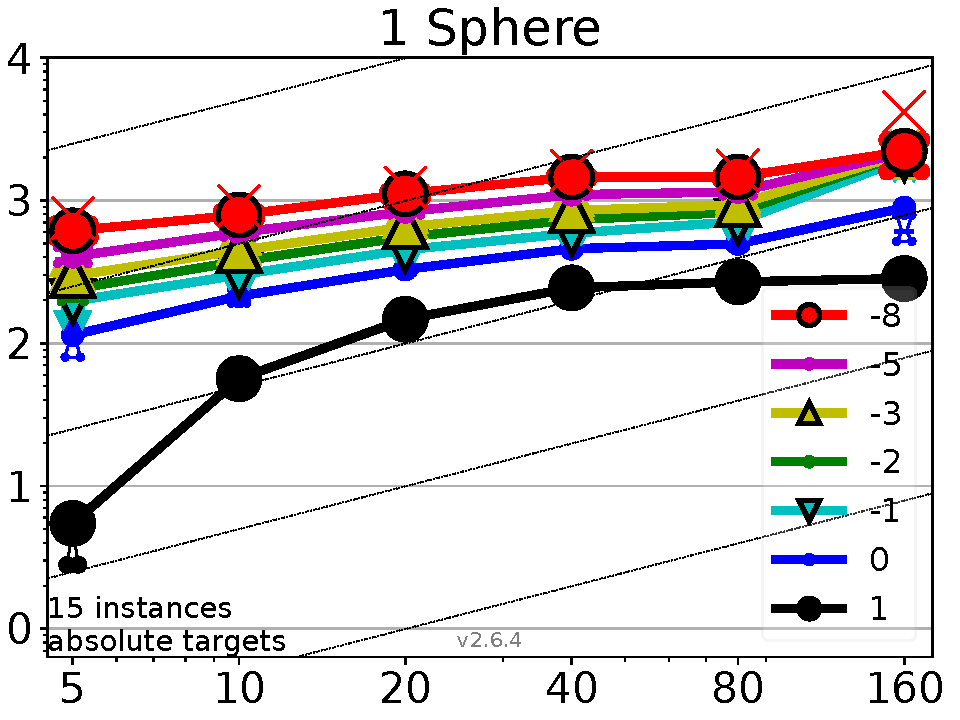
\includegraphics[width=0.24\textwidth]{ppfigdim_f001}&
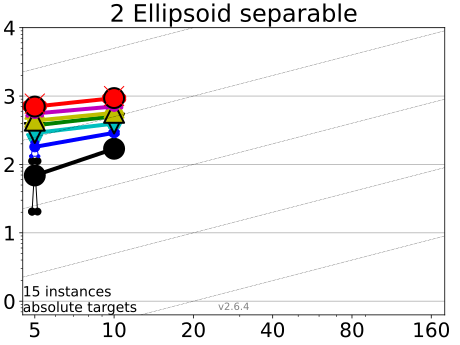
\includegraphics[width=0.24\textwidth]{ppfigdim_f002}&
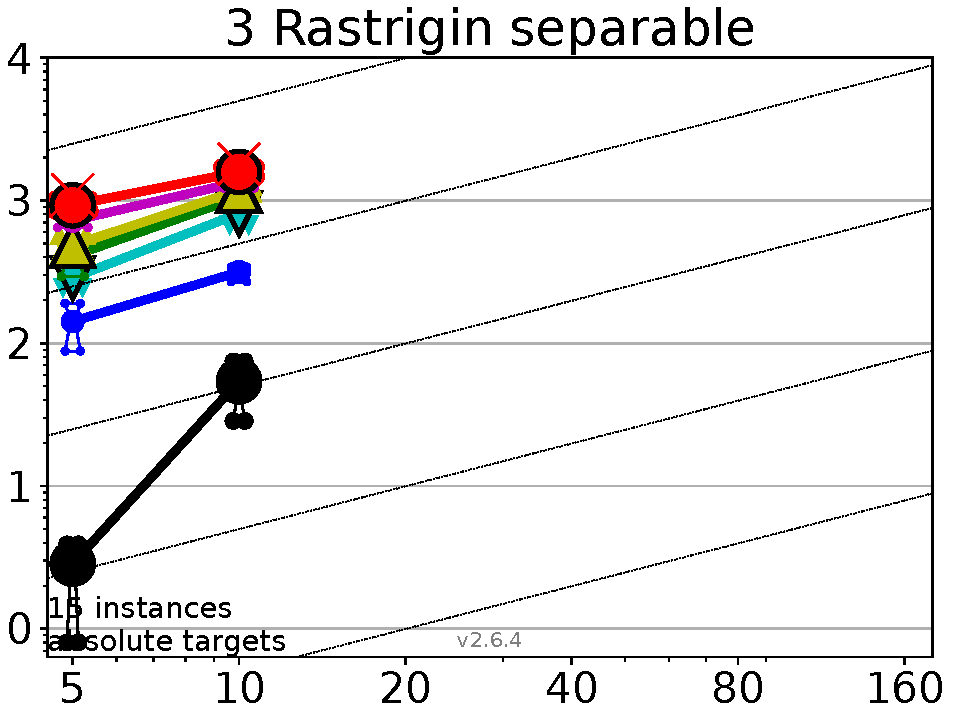
\includegraphics[width=0.24\textwidth]{ppfigdim_f003}&
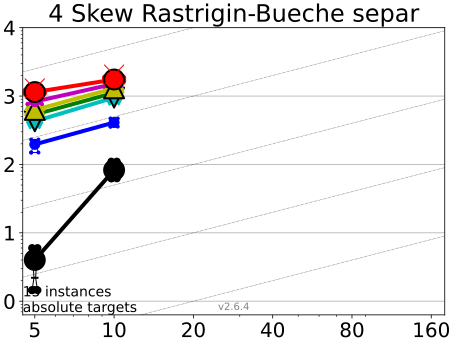
\includegraphics[width=0.24\textwidth]{ppfigdim_f004}\\[-1ex]
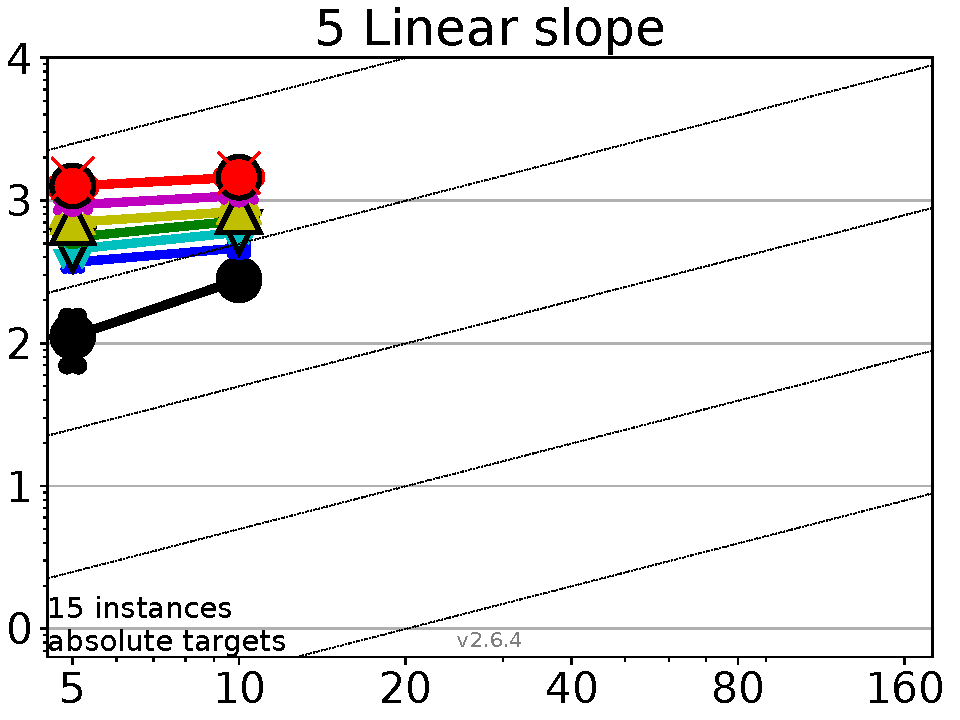
\includegraphics[width=0.24\textwidth]{ppfigdim_f005}&
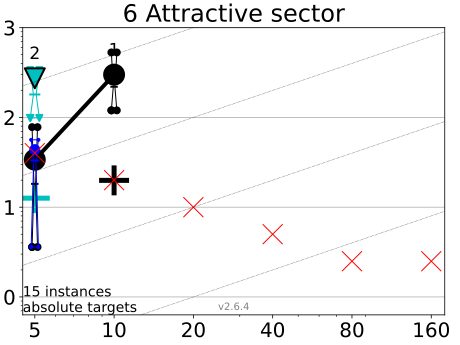
\includegraphics[width=0.24\textwidth]{ppfigdim_f006}&
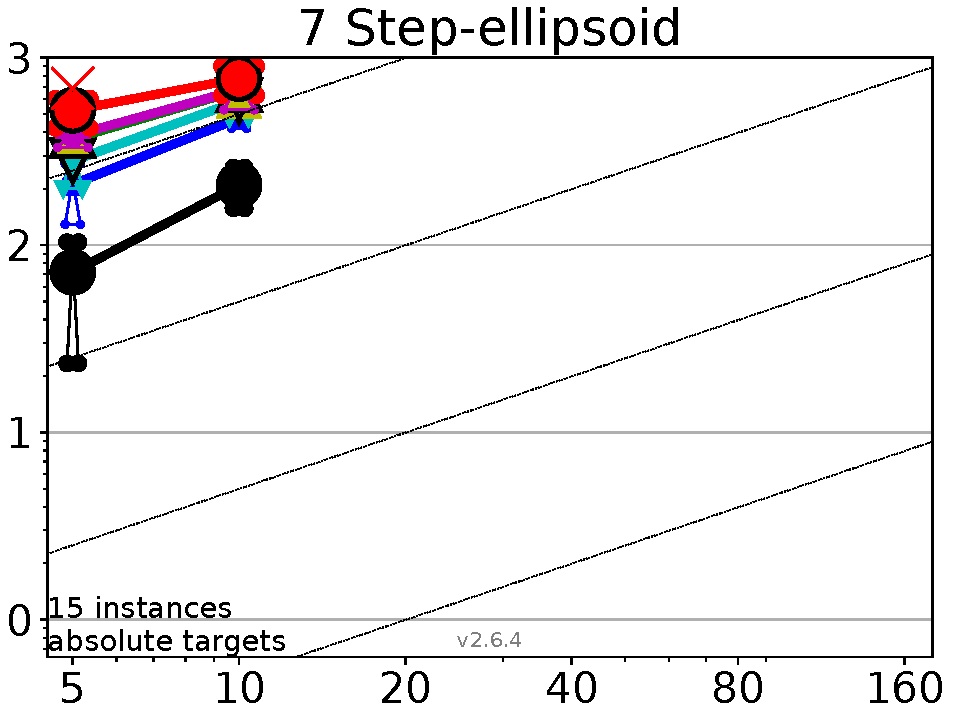
\includegraphics[width=0.24\textwidth]{ppfigdim_f007}&
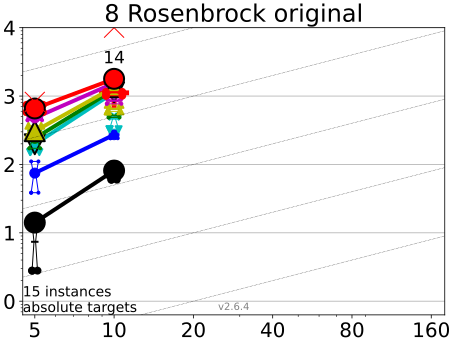
\includegraphics[width=0.24\textwidth]{ppfigdim_f008}\\[-1ex]
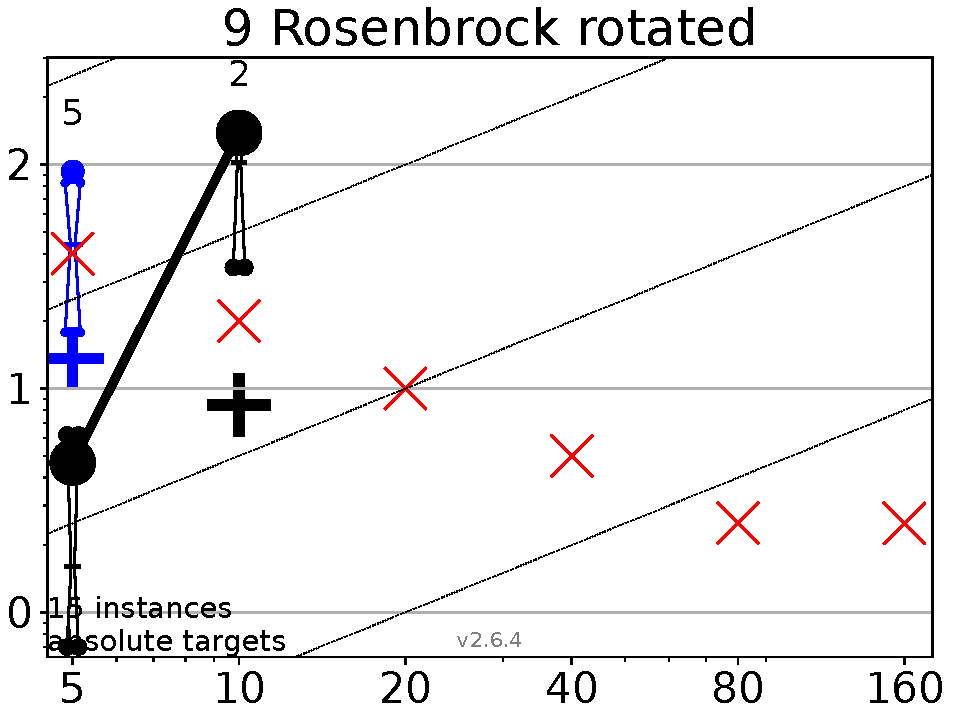
\includegraphics[width=0.24\textwidth]{ppfigdim_f009}&
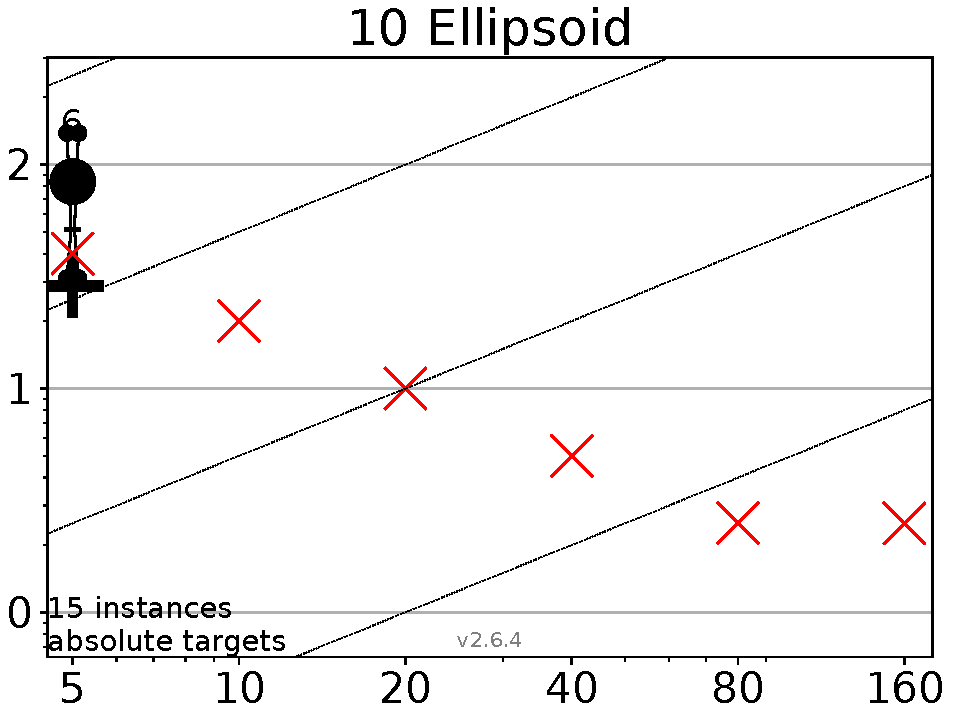
\includegraphics[width=0.24\textwidth]{ppfigdim_f010}&
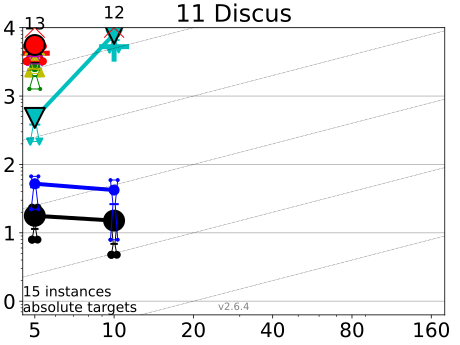
\includegraphics[width=0.24\textwidth]{ppfigdim_f011}&
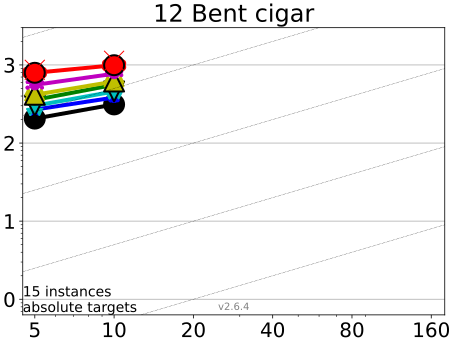
\includegraphics[width=0.24\textwidth]{ppfigdim_f012}\\[-1ex]
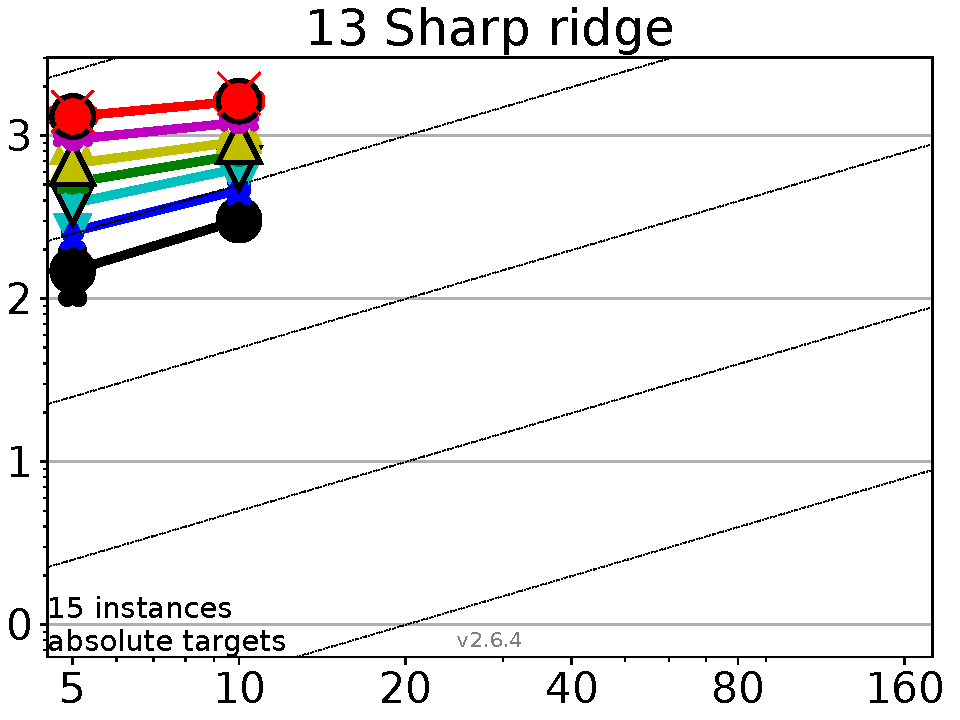
\includegraphics[width=0.24\textwidth]{ppfigdim_f013}&
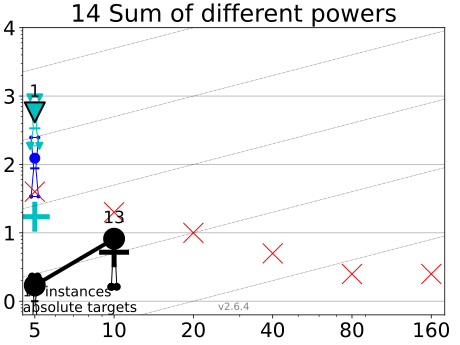
\includegraphics[width=0.24\textwidth]{ppfigdim_f014}&
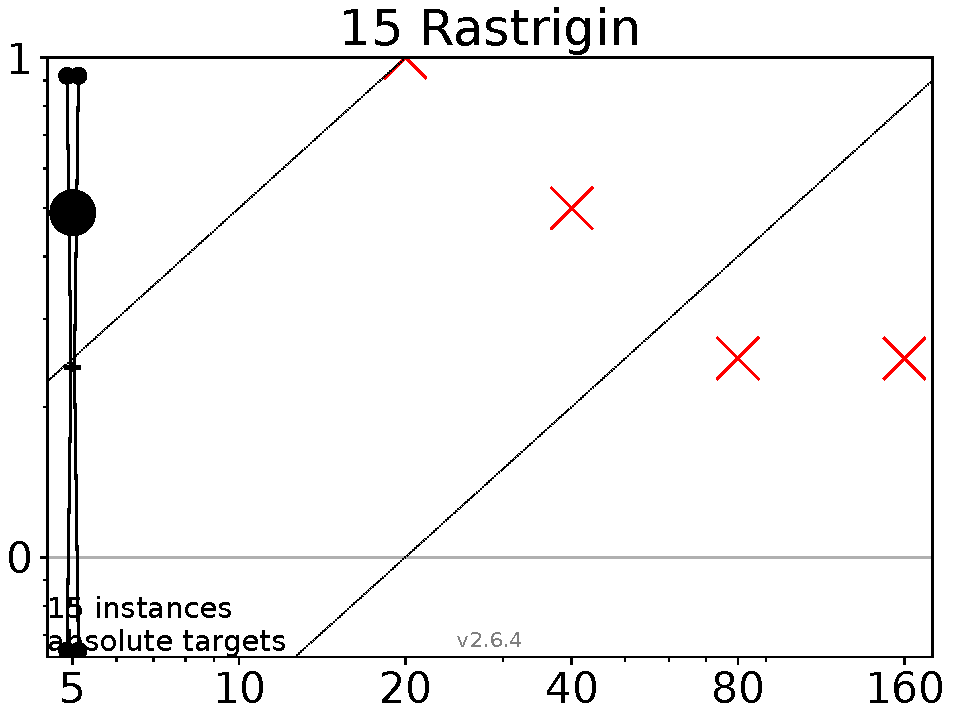
\includegraphics[width=0.24\textwidth]{ppfigdim_f015}&
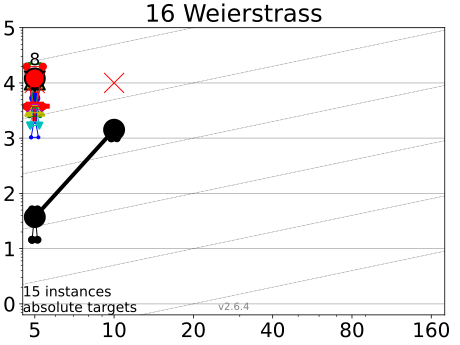
\includegraphics[width=0.24\textwidth]{ppfigdim_f016}\\[-1ex]
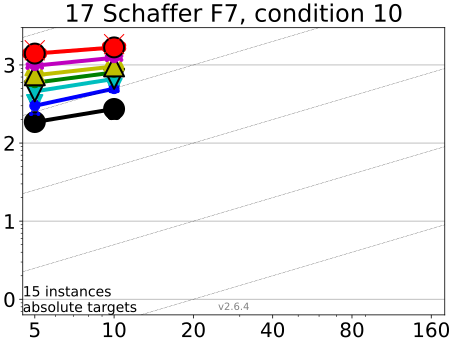
\includegraphics[width=0.24\textwidth]{ppfigdim_f017}&
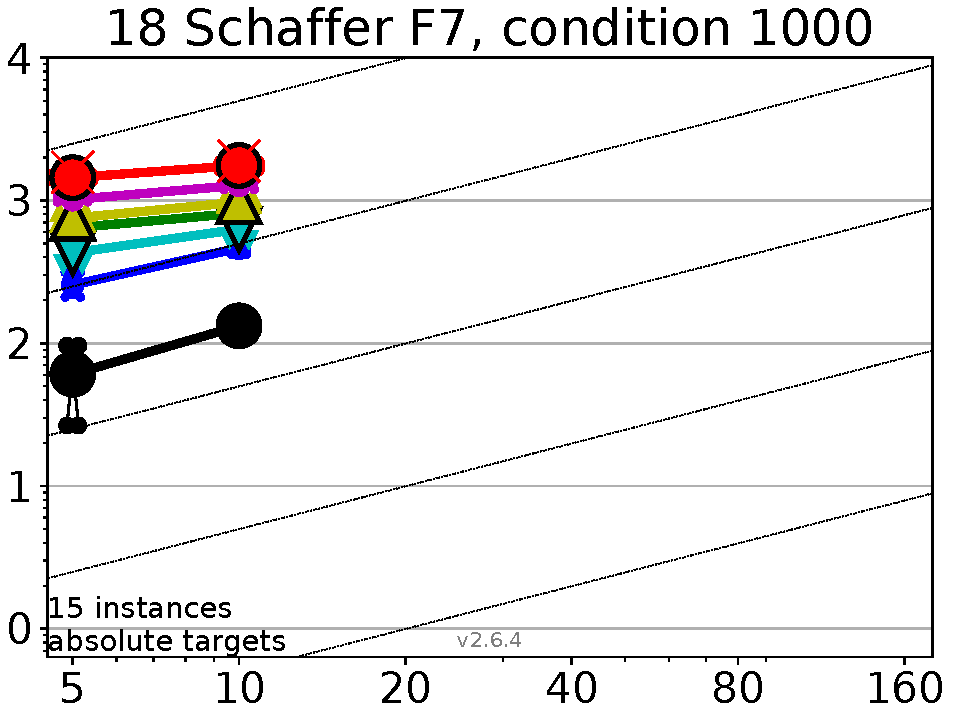
\includegraphics[width=0.24\textwidth]{ppfigdim_f018}&
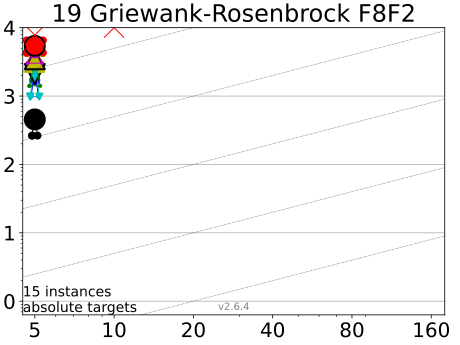
\includegraphics[width=0.24\textwidth]{ppfigdim_f019}&
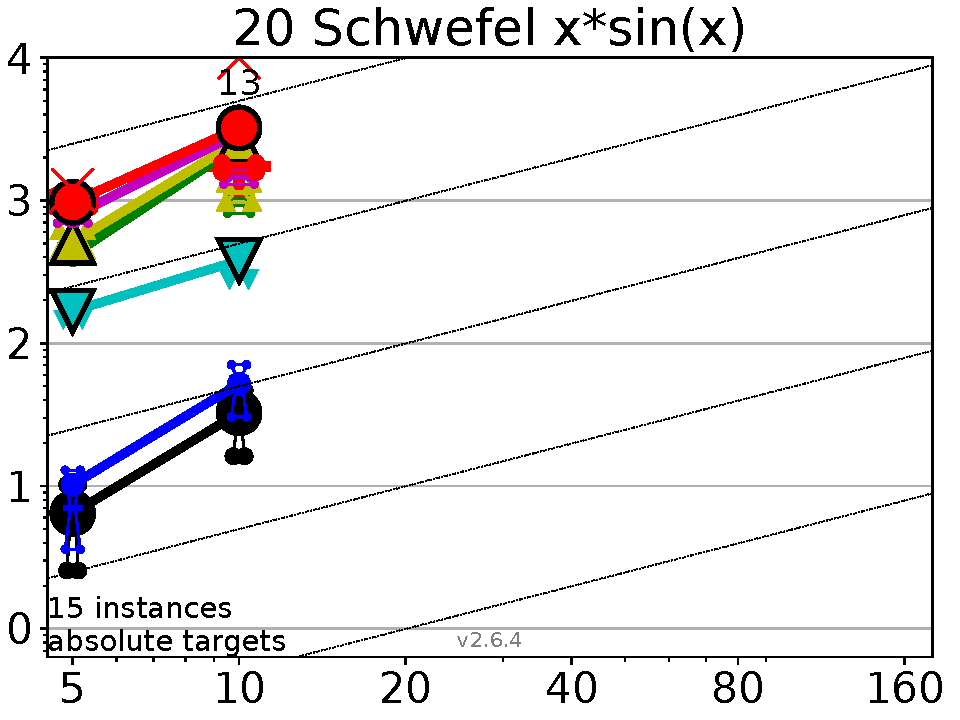
\includegraphics[width=0.24\textwidth]{ppfigdim_f020}\\[-1ex]
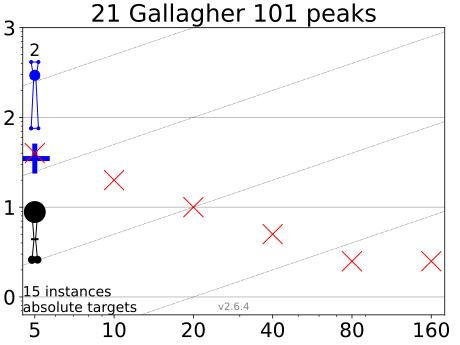
\includegraphics[width=0.24\textwidth]{ppfigdim_f021}&
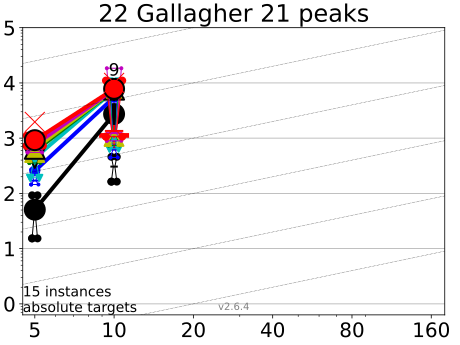
\includegraphics[width=0.24\textwidth]{ppfigdim_f022}&
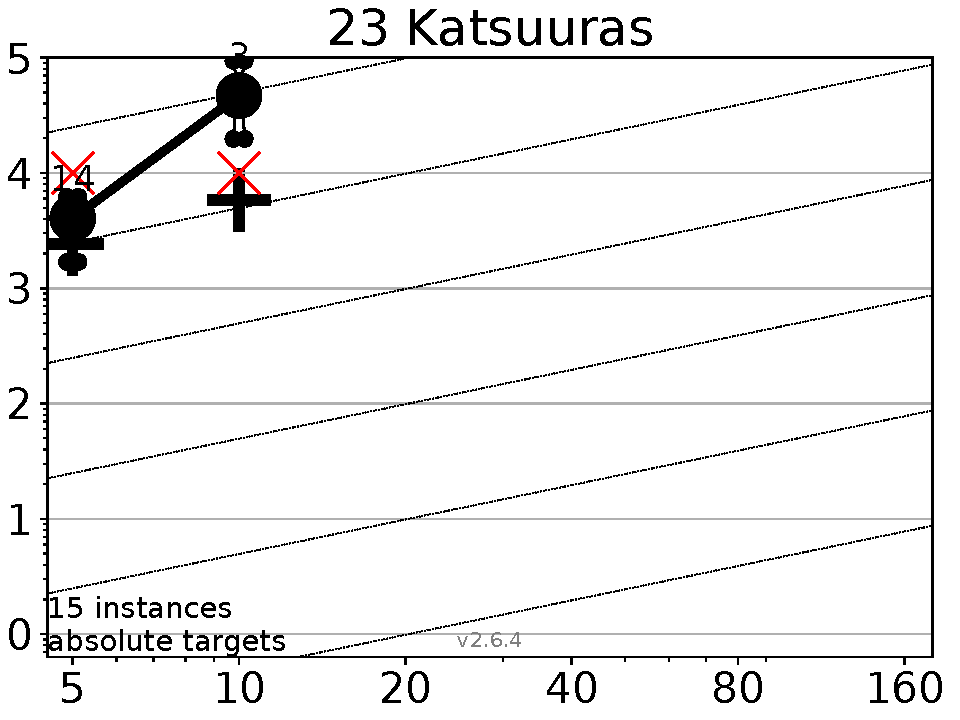
\includegraphics[width=0.24\textwidth]{ppfigdim_f023}&
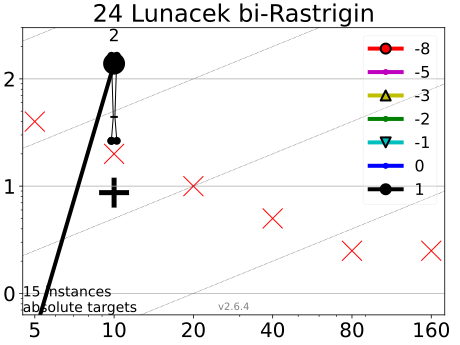
\includegraphics[width=0.24\textwidth]{ppfigdim_f024}
\end{tabular}
\vspace{-3ex}
 \caption{\label{fig:ERTgraphs}
 \bbobppfigdimlegend{$f_1$ and $f_{24}$}
 }
\end{figure*}


%%%%%%%%%%%%%%%%%%%%%%%%%%%%%%%%%%%%%%%%%%%%%%%%%%%%%%%%%%%%%%%%%%%%%%%%%%%%%%%

% ECDFs per group

%%%%%%%%%%%%%%%%%%%%%%%%%%%%%%%%%%%%%%%%%%%%%%%%%%%%%%%%%%%%%%%%%%%%%%%%%%%%%%%

\begin{figure*}
\centering
\begin{tabular}{c@{\hspace*{0.01\textwidth}}c@{\hspace*{0.01\textwidth}}c}
{\sffamily separable fcts}\hspace{1cm} & {\sffamily moderate fcts}\hspace{1cm} & \hspace{-1cm}{\sffamily ill-conditioned fcts}\\
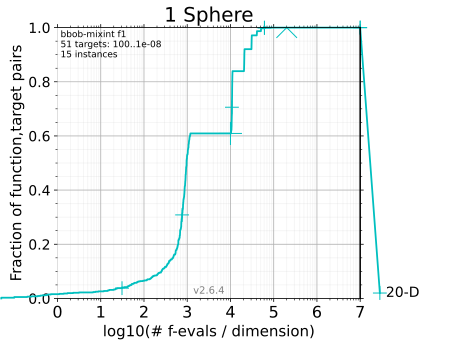
\includegraphics[width=0.32\textwidth]{pprldmany-single-functions/pprldmany_separ}&
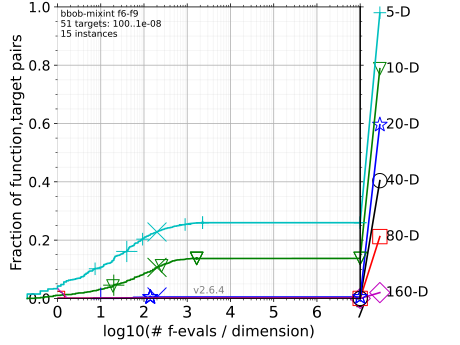
\includegraphics[width=0.32\textwidth]{pprldmany-single-functions/pprldmany_lcond}&
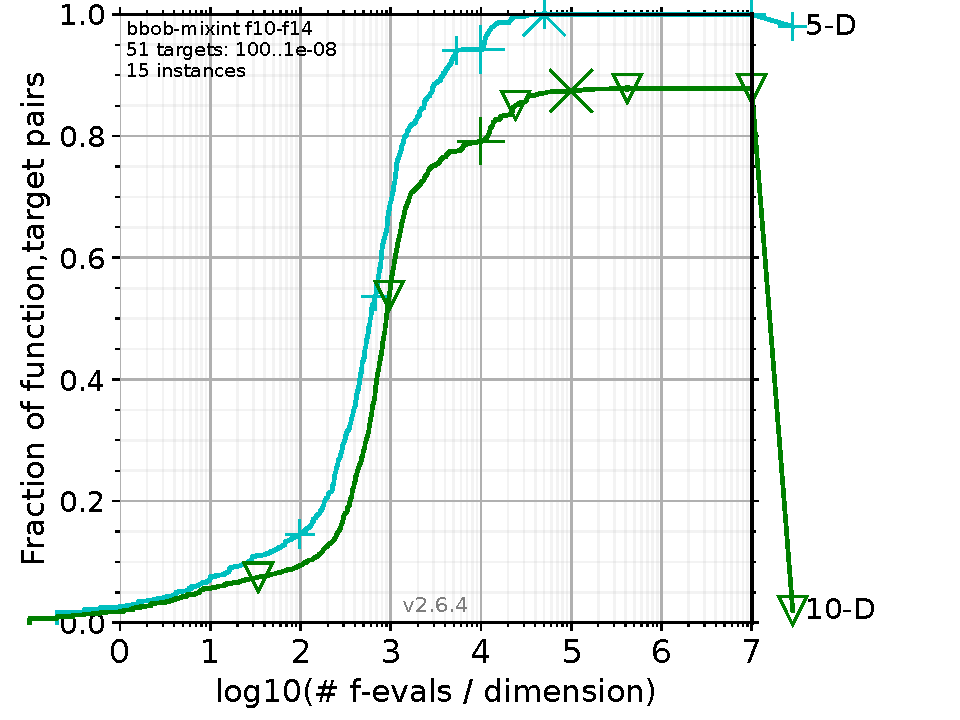
\includegraphics[width=0.32\textwidth]{pprldmany-single-functions/pprldmany_hcond}\\[-0.2em]
{\sffamily multi-modal fcts}\hspace{1cm} & {\sffamily weakly structured multi-modal fcts}\hspace{1cm} & \hspace{-1cm}{\sffamily all fcts}\\
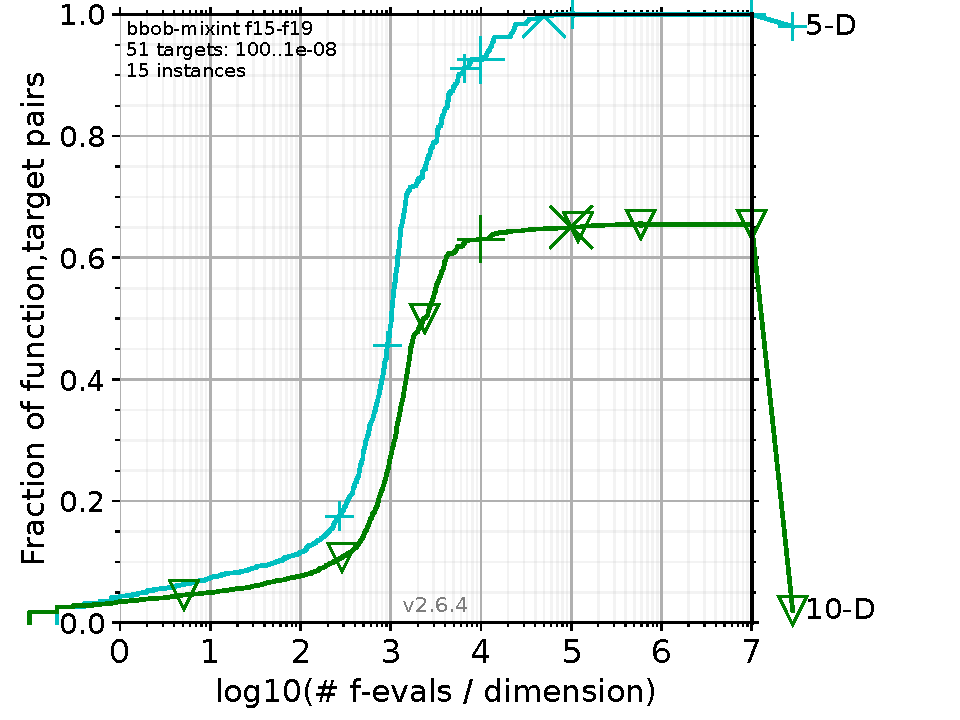
\includegraphics[width=0.32\textwidth]{pprldmany-single-functions/pprldmany_multi}&
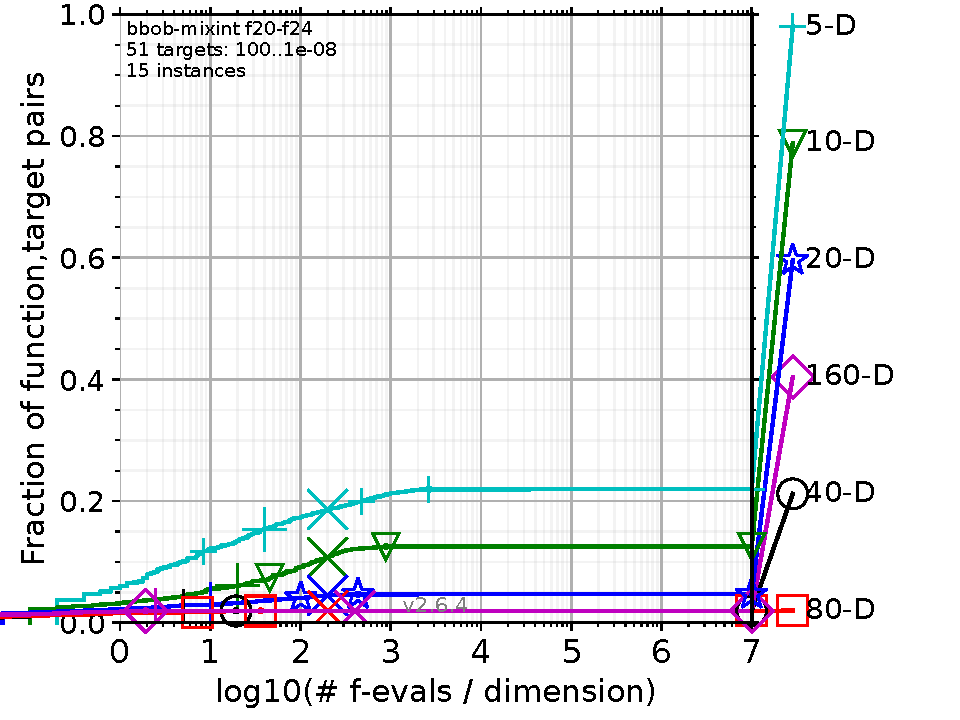
\includegraphics[width=0.32\textwidth]{pprldmany-single-functions/pprldmany_mult2}&
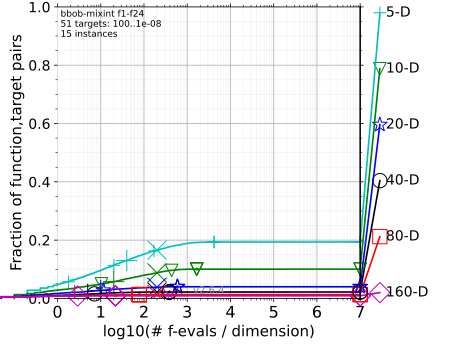
\includegraphics[width=0.32\textwidth]{pprldmany-single-functions/pprldmany}
\vspace*{-1ex}
\end{tabular}
 \caption{\label{fig:ECDFgroups}
	\bbobecdfcaptionallgroups
}
\end{figure*}




%%%%%%%%%%%%%%%%%%%%%%%%%%%%%%%%%%%%%%%%%%%%%%%%%%%%%%%%%%%%%%%%%%%%%%%%%%%%%%%

% ECDFs per function

%%%%%%%%%%%%%%%%%%%%%%%%%%%%%%%%%%%%%%%%%%%%%%%%%%%%%%%%%%%%%%%%%%%%%%%%%%%%%%%

\begin{figure*}
\centering
\begin{tabular}{l@{\hspace*{-0.00\textwidth}}l@{\hspace*{0.01\textwidth}}l@{\hspace*{-0.00\textwidth}}l}
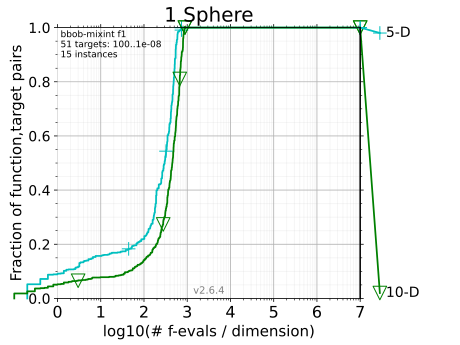
\includegraphics[width=0.24\textwidth]{pprldmany-single-functions/pprldmany_f001}&
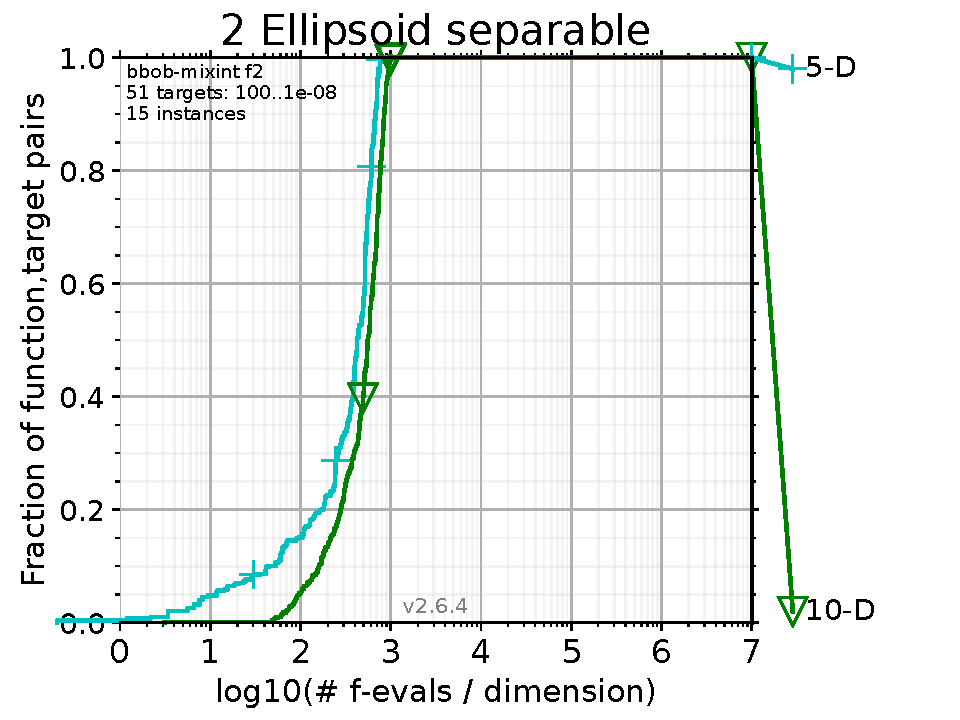
\includegraphics[width=0.24\textwidth]{pprldmany-single-functions/pprldmany_f002}&
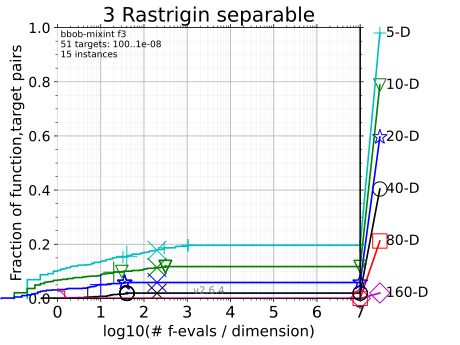
\includegraphics[width=0.24\textwidth]{pprldmany-single-functions/pprldmany_f003}&
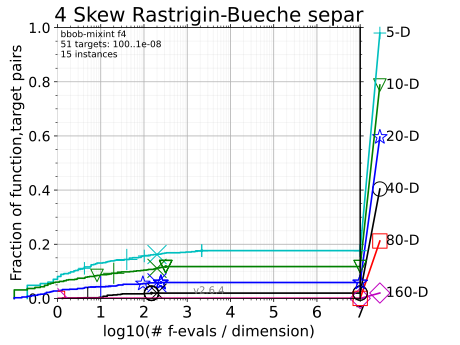
\includegraphics[width=0.24\textwidth]{pprldmany-single-functions/pprldmany_f004}\\[-0.2em]
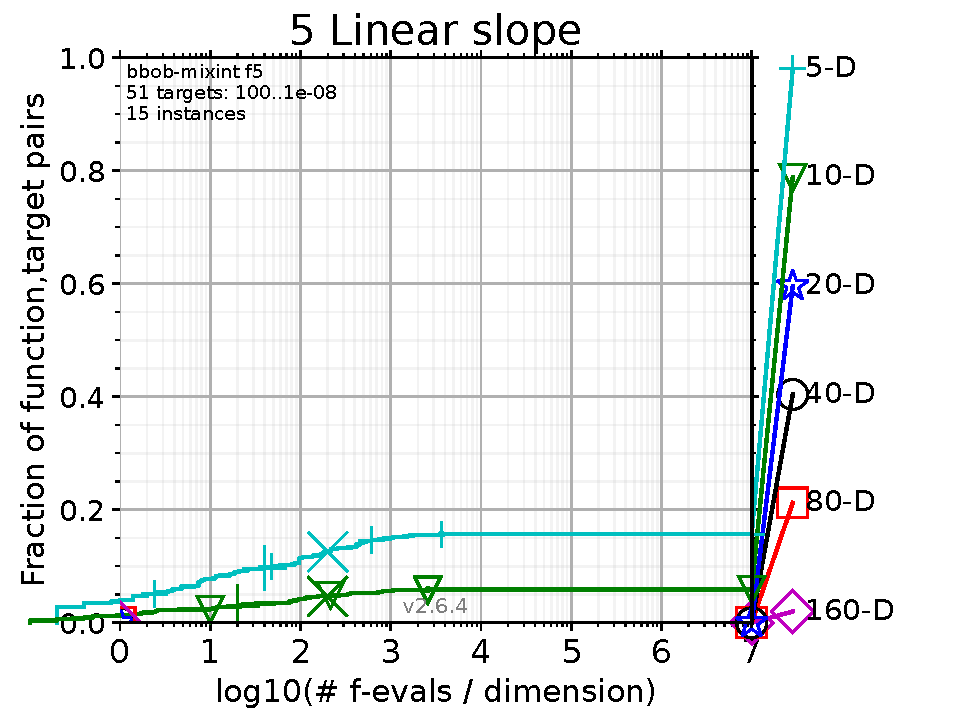
\includegraphics[width=0.24\textwidth]{pprldmany-single-functions/pprldmany_f005}&
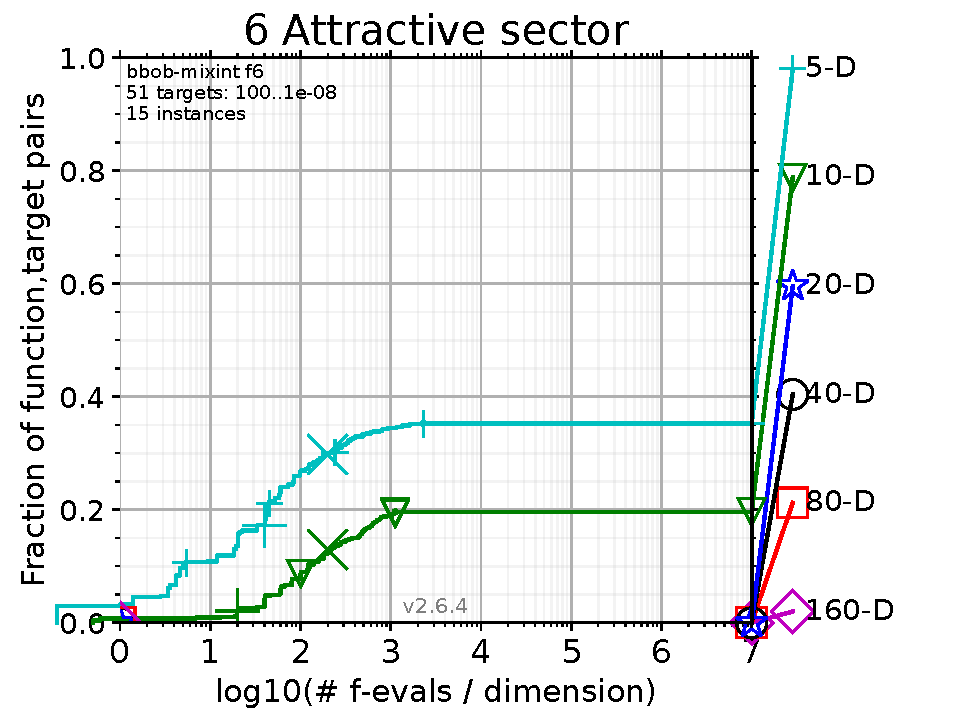
\includegraphics[width=0.24\textwidth]{pprldmany-single-functions/pprldmany_f006}&
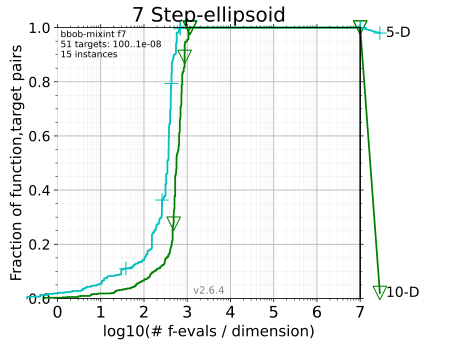
\includegraphics[width=0.24\textwidth]{pprldmany-single-functions/pprldmany_f007}&
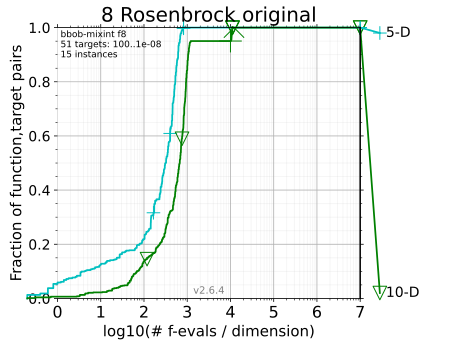
\includegraphics[width=0.24\textwidth]{pprldmany-single-functions/pprldmany_f008}\\[-0.2em]
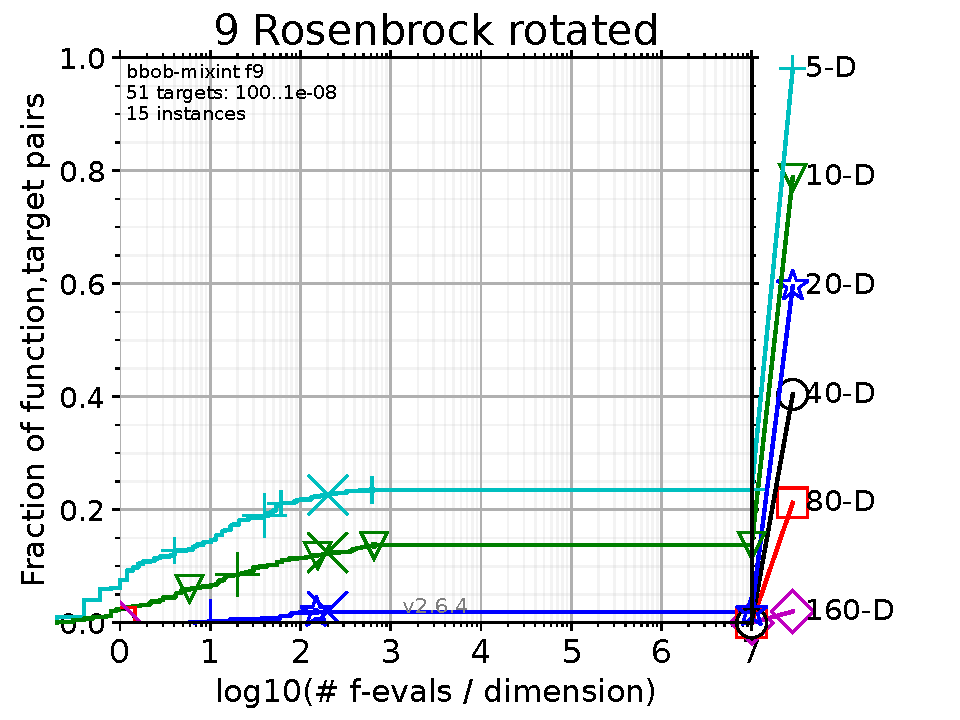
\includegraphics[width=0.24\textwidth]{pprldmany-single-functions/pprldmany_f009}&
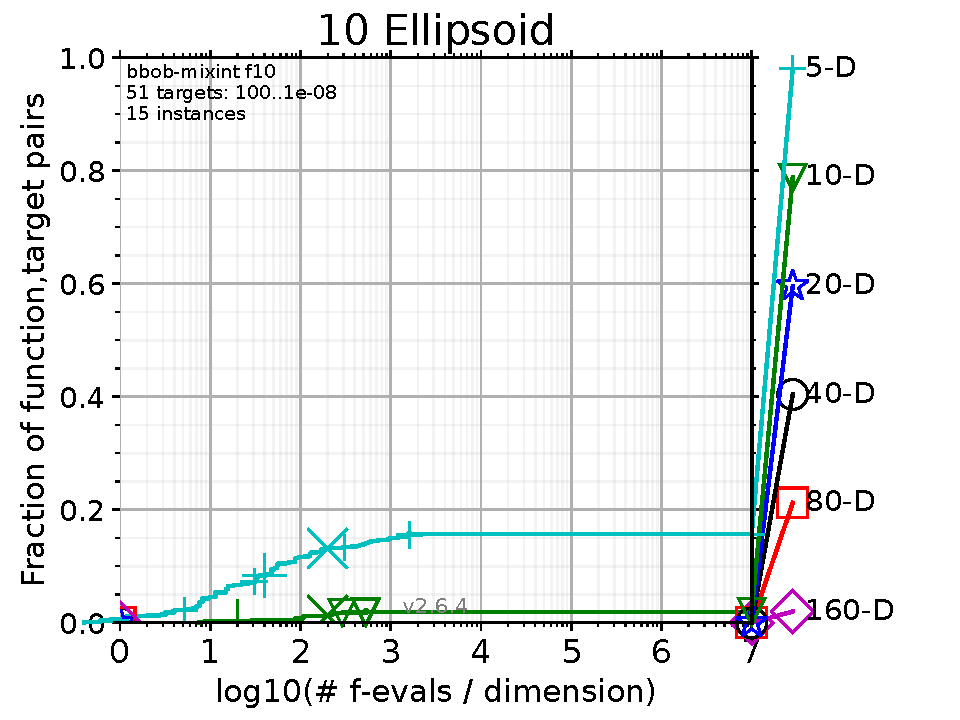
\includegraphics[width=0.24\textwidth]{pprldmany-single-functions/pprldmany_f010}&
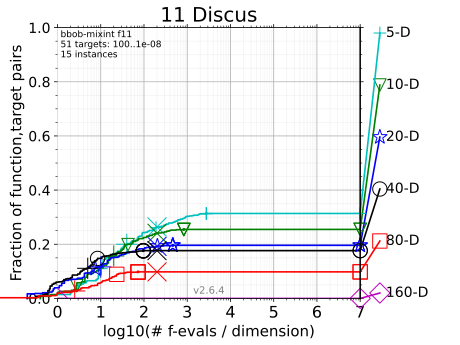
\includegraphics[width=0.24\textwidth]{pprldmany-single-functions/pprldmany_f011}&
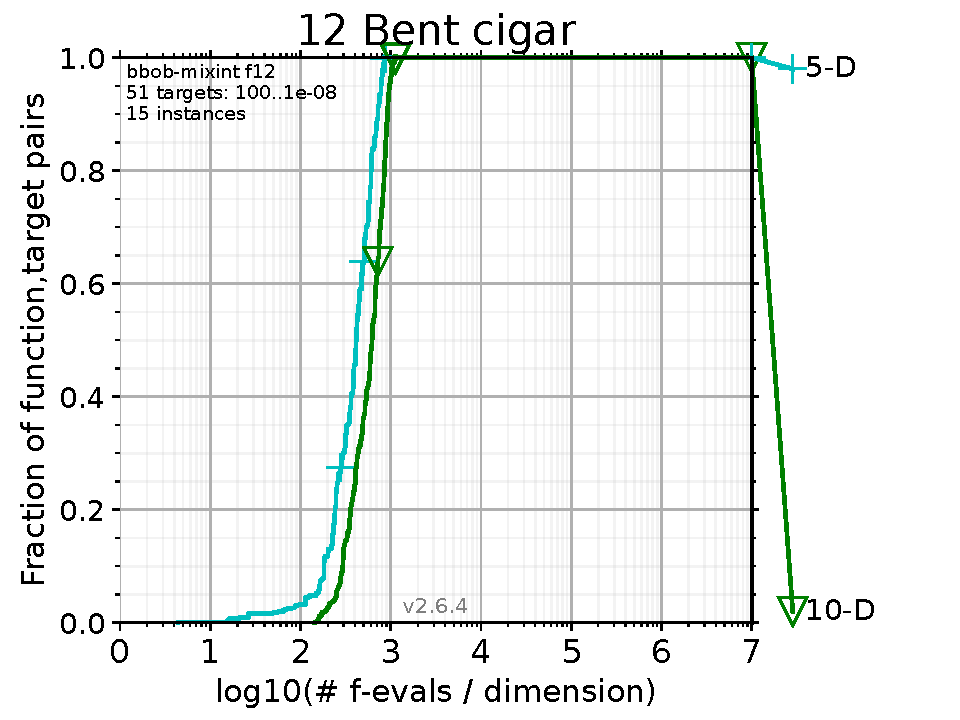
\includegraphics[width=0.24\textwidth]{pprldmany-single-functions/pprldmany_f012}\\[-0.2em]
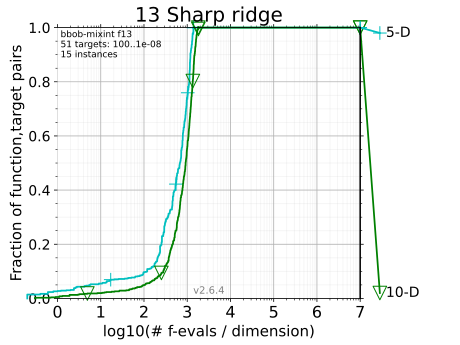
\includegraphics[width=0.24\textwidth]{pprldmany-single-functions/pprldmany_f013}&
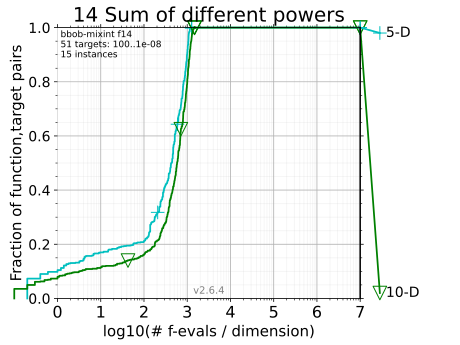
\includegraphics[width=0.24\textwidth]{pprldmany-single-functions/pprldmany_f014}&
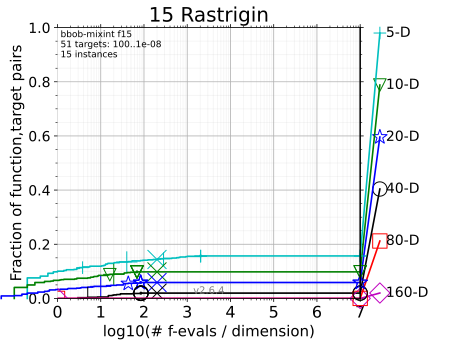
\includegraphics[width=0.24\textwidth]{pprldmany-single-functions/pprldmany_f015}&
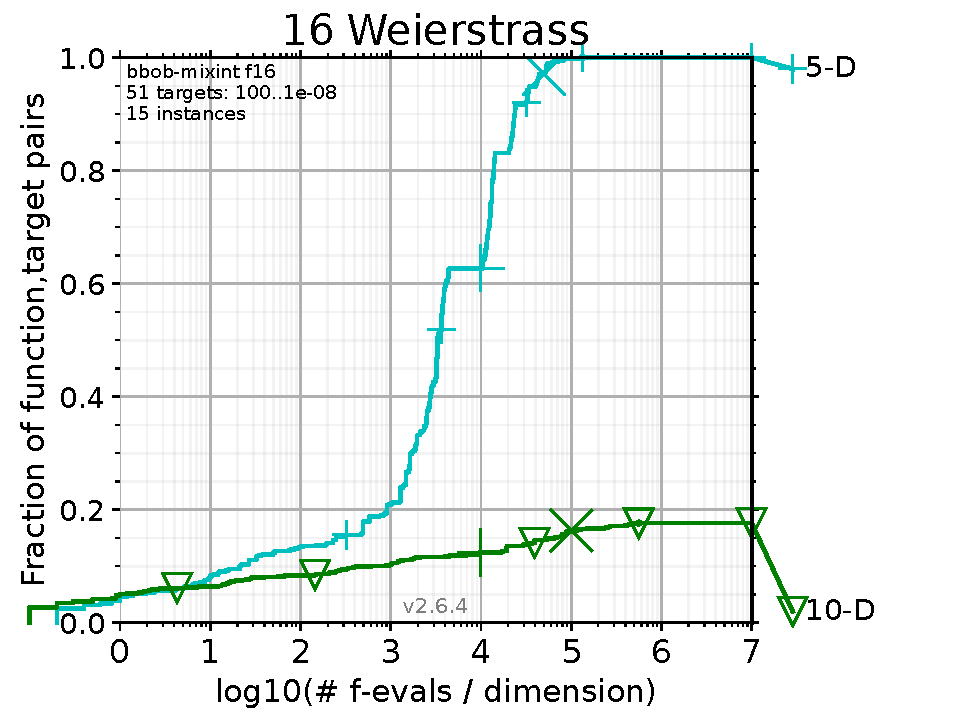
\includegraphics[width=0.24\textwidth]{pprldmany-single-functions/pprldmany_f016}\\[-0.2em]
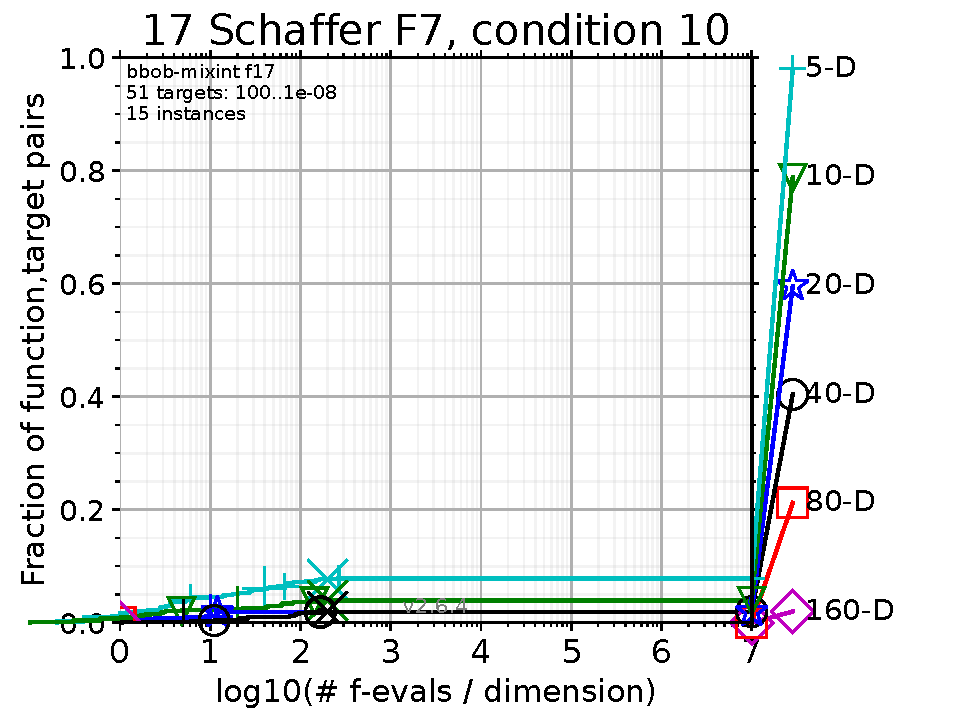
\includegraphics[width=0.24\textwidth]{pprldmany-single-functions/pprldmany_f017}&
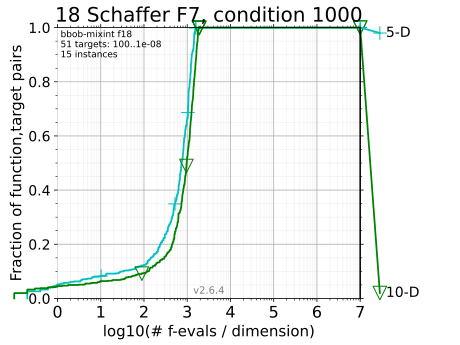
\includegraphics[width=0.24\textwidth]{pprldmany-single-functions/pprldmany_f018}&
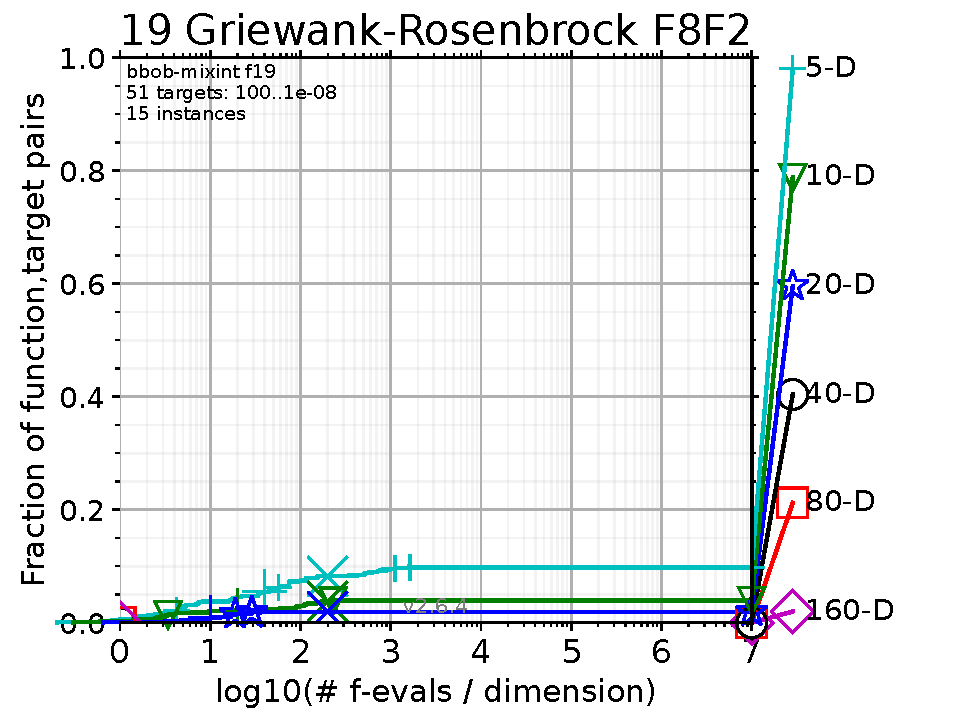
\includegraphics[width=0.24\textwidth]{pprldmany-single-functions/pprldmany_f019}&
\includegraphics[width=0.24\textwidth]{pprldmany-single-functions/pprldmany_f020}\\[-0.2em]
\includegraphics[width=0.24\textwidth]{pprldmany-single-functions/pprldmany_f021}&
\includegraphics[width=0.24\textwidth]{pprldmany-single-functions/pprldmany_f022}&
\includegraphics[width=0.24\textwidth]{pprldmany-single-functions/pprldmany_f023}&
\includegraphics[width=0.24\textwidth]{pprldmany-single-functions/pprldmany_f024}
\vspace*{-1ex}
\end{tabular}
 \caption{\label{fig:ECDFsingleOne}
	\bbobecdfcaptionsinglefunctionssingledim{$\!\!$s 2 to 40}
}
\end{figure*}




%%%%%%%%%%%%%%%%%%%%%%%%%%%%%%%%%%%%%%%%%%%%%%%%%%%%%%%%%%%%%%%%%%%%%%%%%%%%%%%
%%%%%%%%%%%%%%%%%%%%%%%%%%%%%%%%%%%%%%%%%%%%%%%%%%%%%%%%%%%%%%%%%%%%%%%%%%%%%%%%
%
%% ERT loss ratios (figure and table)
%
%%%%%%%%%%%%%%%%%%%%%%%%%%%%%%%%%%%%%%%%%%%%%%%%%%%%%%%%%%%%%%%%%%%%%%%%%%%%%%%%
\begin{figure}
\centering
\parbox{0.48\columnwidth}{\centering 5-D}\hfill
\parbox{0.48\columnwidth}{\centering 20-D}\\
\includegraphics[width=0.48\columnwidth]{pplogloss_05D_noiselessall}\hfill
\includegraphics[width=0.48\columnwidth]{pplogloss_20D_noiselessall}\\[2ex]
%
\input{\bbobdatapath\algfolder pploglosstable_05D_noiselessall}\\
\input{\bbobdatapath\algfolder pploglosstable_20D_noiselessall}
\caption{\label{tab:ERTloss}%
\bbobloglosstablecaption{}
\cocoversion
}
\end{figure}


%%%%%%%%%%%%%%%%%%%%%%%%%%%%%%%%%%%%%%%%%%%%%%%%%%%%%%%%%%%%%%%%%%%%%%%%%%%%%%%
%%%%%%%%%%%%%%%%%%%%%%%%%%%%%%%%%%%%%%%%%%%%%%%%%%%%%%%%%%%%%%%%%%%%%%%%%%%%%%%%
%
%% ERT loss ratios per function group
%
%%%%%%%%%%%%%%%%%%%%%%%%%%%%%%%%%%%%%%%%%%%%%%%%%%%%%%%%%%%%%%%%%%%%%%%%%%%%%%%%
\begin{figure}
\begin{tabular}{@{}l@{}@{}l@{}}
\multicolumn{1}{c}{5-D} & \multicolumn{1}{c}{20-D}\\
\rot[2.8]{separable fcts}
\hspace*{-1.4mm}
\includegraphics[width=0.24\textwidth]{pplogloss_05D_separ} &
\includegraphics[width=0.24\textwidth]{pplogloss_20D_separ}\\
\rot[2.7]{moderate fcts}
\hspace*{-1.4mm}
\includegraphics[width=0.24\textwidth]{pplogloss_05D_lcond} &
\includegraphics[width=0.24\textwidth]{pplogloss_20D_lcond}\\
\rot[1.9]{ill-conditioned fcts}
\hspace*{-1.35mm}
\includegraphics[width=0.24\textwidth]{pplogloss_05D_hcond} &
\includegraphics[width=0.24\textwidth]{pplogloss_20D_hcond}\\
\rot[2.5]{multi-modal fcts}
\hspace*{-1.3mm}
\includegraphics[width=0.24\textwidth]{pplogloss_05D_multi} &
\includegraphics[width=0.24\textwidth]{pplogloss_20D_multi}\\
\rot[1.6]{weak structure fcts}
\hspace*{-1.4mm}
\includegraphics[width=0.24\textwidth]{pplogloss_05D_mult2} &
\includegraphics[width=0.24\textwidth]{pplogloss_20D_mult2}
\vspace*{-0.5ex}
\end{tabular}
 \caption{\label{fig:ERTlogloss}%
\bbobloglossfigurecaption{}
}
\end{figure}

%%%%%%%%%%%%%%%%%%%%%%%%%%%%%%%%%%%%%%%%%%%%%%%%%%%%%%%%%%%%%%%%%%%%%%%%%%%%%%%

%%%%%%%%%%%%%%%%%%%%%%%%%%%%%%%%%%%%%%%%%%%%%%%%%%%%%%%%%%%%%%%%%%%%%%%%%%%%%%%
 
% Table showing the expected runtime (ERT in number of function
% evaluations) divided by the best ERT measured during BBOB-2009 (given in the
% first row of each cell) for functions $f_1$--$f_{24} for dimension 5$.

%%%%%%%%%%%%%%%%%%%%%%%%%%%%%%%%%%%%%%%%%%%%%%%%%%%%%%%%%%%%%%%%%%%%%%%%%%%%%%%

\begin{table*}\tiny
%\hfill10-D\hfill~\\[1ex]
{\normalsize \color{red}
\ifthenelse{\isundefined{\algorithmG}}{}{more than 6 algorithms: please split the tables below by hand until it fits to the page limits}
}
\mbox{\begin{minipage}[t]{0.499\textwidth}\tiny
\centering
\pptableheader 

\input{\bbobdatapath\algfolder pptable_f001_05D} 

\input{\bbobdatapath\algfolder pptable_f002_05D}

\input{\bbobdatapath\algfolder pptable_f003_05D}

\input{\bbobdatapath\algfolder pptable_f004_05D}

\input{\bbobdatapath\algfolder pptable_f005_05D}

\input{\bbobdatapath\algfolder pptable_f006_05D}

\input{\bbobdatapath\algfolder pptable_f007_05D}

\input{\bbobdatapath\algfolder pptable_f008_05D}

\input{\bbobdatapath\algfolder pptable_f009_05D}

\input{\bbobdatapath\algfolder pptable_f010_05D}

\input{\bbobdatapath\algfolder pptable_f011_05D}

\input{\bbobdatapath\algfolder pptable_f012_05D}

\pptablefooter

\end{minipage}
\hspace{0.002\textwidth}
\begin{minipage}[t]{0.499\textwidth}\tiny
\centering

\pptableheader 

\input{\bbobdatapath\algfolder pptable_f013_05D}

\input{\bbobdatapath\algfolder pptable_f014_05D}

\input{\bbobdatapath\algfolder pptable_f015_05D}

\input{\bbobdatapath\algfolder pptable_f016_05D}

\input{\bbobdatapath\algfolder pptable_f017_05D}

\input{\bbobdatapath\algfolder pptable_f018_05D}

\input{\bbobdatapath\algfolder pptable_f019_05D}

\input{\bbobdatapath\algfolder pptable_f020_05D}

\input{\bbobdatapath\algfolder pptable_f021_05D}

\input{\bbobdatapath\algfolder pptable_f022_05D}

\input{\bbobdatapath\algfolder pptable_f023_05D}

\input{\bbobdatapath\algfolder pptable_f024_05D}

\pptablefooter

\end{minipage}}

\caption[Table of ERTs]{\label{tab:ERTs05}\bbobpptablecaption{dimension $5$}
\cocoversion
}
\end{table*}

%%%%%%%%%%%%%%%%%%%%%%%%%%%%%%%%%%%%%%%%%%%%%%%%%%%%%%%%%%%%%%%%%%%%%%%%%%%%%%%

%%%%%%%%%%%%%%%%%%%%%%%%%%%%%%%%%%%%%%%%%%%%%%%%%%%%%%%%%%%%%%%%%%%%%%%%%%%%%%%
 
% Table showing the expected runtime (ERT in number of function
% evaluations) [divided by the best ERT measured during BBOB-2009] (given in the
% first row of each cell) for functions $f_1$--$f_{24} for dimension 20$.

%%%%%%%%%%%%%%%%%%%%%%%%%%%%%%%%%%%%%%%%%%%%%%%%%%%%%%%%%%%%%%%%%%%%%%%%%%%%%%%

\begin{table*}\tiny
%\hfill20-D\hfill~\\[1ex]
{\normalsize \color{red}
\ifthenelse{\isundefined{\algorithmG}}{}{more than 6 algorithms: please split the tables below by hand until it fits to the page limits}
}
\mbox{\begin{minipage}[t]{0.499\textwidth}\tiny
\centering
\pptableheader 

\input{\bbobdatapath\algfolder pptable_f001_20D} 

\input{\bbobdatapath\algfolder pptable_f002_20D}

\input{\bbobdatapath\algfolder pptable_f003_20D}

\input{\bbobdatapath\algfolder pptable_f004_20D}

\input{\bbobdatapath\algfolder pptable_f005_20D}

\input{\bbobdatapath\algfolder pptable_f006_20D}

\input{\bbobdatapath\algfolder pptable_f007_20D}

\input{\bbobdatapath\algfolder pptable_f008_20D}

\input{\bbobdatapath\algfolder pptable_f009_20D}

\input{\bbobdatapath\algfolder pptable_f010_20D}

\input{\bbobdatapath\algfolder pptable_f011_20D}

\input{\bbobdatapath\algfolder pptable_f012_20D}

\pptablefooter

\end{minipage}
\hspace{0.002\textwidth}
\begin{minipage}[t]{0.499\textwidth}\tiny
\centering

\pptableheader 

\input{\bbobdatapath\algfolder pptable_f013_20D}

\input{\bbobdatapath\algfolder pptable_f014_20D}

\input{\bbobdatapath\algfolder pptable_f015_20D}

\input{\bbobdatapath\algfolder pptable_f016_20D}

\input{\bbobdatapath\algfolder pptable_f017_20D}

\input{\bbobdatapath\algfolder pptable_f018_20D}

\input{\bbobdatapath\algfolder pptable_f019_20D}

\input{\bbobdatapath\algfolder pptable_f020_20D}

\input{\bbobdatapath\algfolder pptable_f021_20D}

\input{\bbobdatapath\algfolder pptable_f022_20D}

\input{\bbobdatapath\algfolder pptable_f023_20D}

\input{\bbobdatapath\algfolder pptable_f024_20D}

\pptablefooter

\end{minipage}}

\caption[Table of ERTs]{\label{tab:ERTs20}\bbobpptablecaption{dimension $20$}
\cocoversion
}
\end{table*}

%%%%%%%%%%%%%%%%%%%%%%%%%%%%%%%%%%%%%%%%%%%%%%%%%%%%%%%%%%%%%%%%%%%%%%%%%%%%%%%


}{} % end of 1 algorithm template



\ifthenelse{\numofalgs > 1}{

%%%%%%%%%%%%%%%%%%%%%%%%%%%%%%%%%%%%%%%%%%%%%%%%%%%%%%%%%%%%%%%%%%%%%%%%%%%%%%%
%%%%%%%%%%%%%%%%%%%%%%%%%%%%%%%%%%%%%%%%%%%%%%%%%%%%%%%%%%%%%%%%%%%%%%%%%%%%%%%

% Scaling of ERT with dimension

%%%%%%%%%%%%%%%%%%%%%%%%%%%%%%%%%%%%%%%%%%%%%%%%%%%%%%%%%%%%%%%%%%%%%%%%%%%%%%%

\begin{figure*}
\centering
\begin{tabular}{@{}c@{}c@{}c@{}c@{}}
\includegraphics[width=0.24\textwidth]{ppfigs_f001}&
\includegraphics[width=0.24\textwidth]{ppfigs_f002}&
\includegraphics[width=0.24\textwidth]{ppfigs_f003}&
\includegraphics[width=0.24\textwidth]{ppfigs_f004}\\[-0.25em]
\includegraphics[width=0.24\textwidth]{ppfigs_f005}&
\includegraphics[width=0.24\textwidth]{ppfigs_f006}&
\includegraphics[width=0.24\textwidth]{ppfigs_f007}&
\includegraphics[width=0.24\textwidth]{ppfigs_f008}\\[-0.25em]
\includegraphics[width=0.24\textwidth]{ppfigs_f009}&
\includegraphics[width=0.24\textwidth]{ppfigs_f010}&
\includegraphics[width=0.24\textwidth]{ppfigs_f011}&
\includegraphics[width=0.24\textwidth]{ppfigs_f012}\\[-0.25em]
\includegraphics[width=0.24\textwidth]{ppfigs_f013}&
\includegraphics[width=0.24\textwidth]{ppfigs_f014}&
\includegraphics[width=0.24\textwidth]{ppfigs_f015}&
\includegraphics[width=0.24\textwidth]{ppfigs_f016}\\[-0.25em]
\includegraphics[width=0.24\textwidth]{ppfigs_f017}&
\includegraphics[width=0.24\textwidth]{ppfigs_f018}&
\includegraphics[width=0.24\textwidth]{ppfigs_f019}&
\includegraphics[width=0.24\textwidth]{ppfigs_f020}\\[-0.25em]
\includegraphics[width=0.24\textwidth]{ppfigs_f021}&
\includegraphics[width=0.24\textwidth]{ppfigs_f022}&
\includegraphics[width=0.24\textwidth]{ppfigs_f023}&
\includegraphics[width=0.24\textwidth]{ppfigs_f024}
\end{tabular}
\vspace*{-0.2cm}
\caption[Expected running time (\ERT) divided by dimension
versus dimension in log-log presentation]{
\label{fig:scaling}
\bbobppfigslegend{$f_1$ and $f_{24}$}. 
}
% 
\end{figure*}







%%%%%%%%%%%%%%%%%%%%%%%%%%%%%%%%%%%%%%%%%%%%%%%%%%%%%%%%%%%%%%%%%%%%%%%%%%%%%%%
%%%%%%%%%%%%%%%%%%%%%%%%%%%%%%%%%%%%%%%%%%%%%%%%%%%%%%%%%%%%%%%%%%%%%%%%%%%%%%%
 
% Empirical cumulative distribution functions (ECDFs) per function group
% for dimensions 5 and 20

%%%%%%%%%%%%%%%%%%%%%%%%%%%%%%%%%%%%%%%%%%%%%%%%%%%%%%%%%%%%%%%%%%%%%%%%%%%%%%%

\begin{figure*}
\begin{tabular}{c@{\hspace*{0.01\textwidth}}c@{\hspace*{0.01\textwidth}}c}
{\sffamily separable fcts}\hspace{1cm} & {\sffamily moderate fcts}\hspace{1cm} & \hspace{-1cm}{\sffamily ill-conditioned fcts}\\
\includegraphics[width=0.32\textwidth]{\bbobdatapath\algsfolder/pprldmany_05D_separ}&
\includegraphics[width=0.32\textwidth]{\bbobdatapath\algsfolder/pprldmany_05D_lcond}&
\includegraphics[width=0.32\textwidth]{\bbobdatapath\algsfolder/pprldmany_05D_hcond}\\[-0.2em]
{\sffamily multi-modal fcts}\hspace{1cm} & {\sffamily weakly structured multi-modal fcts}\hspace{1cm} & \hspace{-1cm}{\sffamily all fcts}\\
\includegraphics[width=0.32\textwidth]{\bbobdatapath\algsfolder/pprldmany_05D_multi}&
\includegraphics[width=0.32\textwidth]{\bbobdatapath\algsfolder/pprldmany_05D_mult2}&
\includegraphics[width=0.32\textwidth]{\bbobdatapath\algsfolder/pprldmany_05D_noiselessall}
\vspace*{-1ex}
\end{tabular}
\caption{
\label{fig:ECDFs05D}
\bbobECDFslegend{5}
}
\end{figure*}


\begin{figure*}
\begin{tabular}{c@{\hspace*{0.01\textwidth}}c@{\hspace*{0.01\textwidth}}c}
{\sffamily separable fcts}\hspace{1cm} & {\sffamily moderate fcts}\hspace{1cm} & \hspace{-1cm}{\sffamily ill-conditioned fcts}\\
\includegraphics[width=0.32\textwidth]{\bbobdatapath\algsfolder/pprldmany_20D_separ}&
\includegraphics[width=0.32\textwidth]{\bbobdatapath\algsfolder/pprldmany_20D_lcond}&
\includegraphics[width=0.32\textwidth]{\bbobdatapath\algsfolder/pprldmany_20D_hcond}\\[-0.2em]
{\sffamily multi-modal fcts}\hspace{1cm} & {\sffamily weakly structured multi-modal fcts}\hspace{1cm} & \hspace{-1cm}{\sffamily all fcts}\\
\includegraphics[width=0.32\textwidth]{\bbobdatapath\algsfolder/pprldmany_20D_multi}&
\includegraphics[width=0.32\textwidth]{\bbobdatapath\algsfolder/pprldmany_20D_mult2}&
\includegraphics[width=0.32\textwidth]{\bbobdatapath\algsfolder/pprldmany_20D_noiselessall}
\vspace*{-1ex}
\end{tabular}
\caption{
\label{fig:ECDFs20D}
\bbobECDFslegend{20}
}
\end{figure*}

%%%%%%%%%%%%%%%%%%%%%%%%%%%%%%%%%%%%%%%%%%%%%%%%%%%%%%%%%%%%%%%%%%%%%%%%%%%%%%%
%%%%%%%%%%%%%%%%%%%%%%%%%%%%%%%%%%%%%%%%%%%%%%%%%%%%%%%%%%%%%%%%%%%%%%%%%%%%%%%

% ECDFs per function in dimension 5

%%%%%%%%%%%%%%%%%%%%%%%%%%%%%%%%%%%%%%%%%%%%%%%%%%%%%%%%%%%%%%%%%%%%%%%%%%%%%%%
\begin{figure*}
\centering
\begin{tabular}{@{}l@{}l@{}l@{}l@{}l@{}}
\includegraphics[width=0.2\textwidth]{pprldmany-single-functions/pprldmany_f001_05D}&
\includegraphics[width=0.2\textwidth]{pprldmany-single-functions/pprldmany_f002_05D}&
\includegraphics[width=0.2\textwidth]{pprldmany-single-functions/pprldmany_f003_05D}&
\includegraphics[width=0.2\textwidth]{pprldmany-single-functions/pprldmany_f004_05D}\\
\includegraphics[width=0.2\textwidth]{pprldmany-single-functions/pprldmany_f005_05D}&
\includegraphics[width=0.2\textwidth]{pprldmany-single-functions/pprldmany_f006_05D}&
\includegraphics[width=0.2\textwidth]{pprldmany-single-functions/pprldmany_f007_05D}&
\includegraphics[width=0.2\textwidth]{pprldmany-single-functions/pprldmany_f008_05D}\\
\includegraphics[width=0.2\textwidth]{pprldmany-single-functions/pprldmany_f009_05D}&
\includegraphics[width=0.2\textwidth]{pprldmany-single-functions/pprldmany_f010_05D}&
\includegraphics[width=0.2\textwidth]{pprldmany-single-functions/pprldmany_f011_05D}&
\includegraphics[width=0.2\textwidth]{pprldmany-single-functions/pprldmany_f012_05D}\\
\includegraphics[width=0.2\textwidth]{pprldmany-single-functions/pprldmany_f013_05D}&
\includegraphics[width=0.2\textwidth]{pprldmany-single-functions/pprldmany_f014_05D}&
\includegraphics[width=0.2\textwidth]{pprldmany-single-functions/pprldmany_f015_05D}&
\includegraphics[width=0.2\textwidth]{pprldmany-single-functions/pprldmany_f016_05D}\\
\includegraphics[width=0.2\textwidth]{pprldmany-single-functions/pprldmany_f017_05D}&
\includegraphics[width=0.2\textwidth]{pprldmany-single-functions/pprldmany_f018_05D}&
\includegraphics[width=0.2\textwidth]{pprldmany-single-functions/pprldmany_f019_05D}&
\includegraphics[width=0.2\textwidth]{pprldmany-single-functions/pprldmany_f020_05D}\\
\includegraphics[width=0.2\textwidth]{pprldmany-single-functions/pprldmany_f021_05D}&
\includegraphics[width=0.2\textwidth]{pprldmany-single-functions/pprldmany_f022_05D}&
\includegraphics[width=0.2\textwidth]{pprldmany-single-functions/pprldmany_f023_05D}&
\includegraphics[width=0.2\textwidth]{pprldmany-single-functions/pprldmany_f024_05D}
\end{tabular}
 \caption{\label{fig:ECDFsingleOne}
	\bbobecdfcaptionsinglefunctionssingledim{5}
}
\end{figure*}


%%%%%%%%%%%%%%%%%%%%%%%%%%%%%%%%%%%%%%%%%%%%%%%%%%%%%%%%%%%%%%%%%%%%%%%%%%%%%%%
%%%%%%%%%%%%%%%%%%%%%%%%%%%%%%%%%%%%%%%%%%%%%%%%%%%%%%%%%%%%%%%%%%%%%%%%%%%%%%%
 
% Table showing the expected runtime (ERT in number of function
% evaluations) for functions $f_1$--$f_{24}$ for dimension 5.

%%%%%%%%%%%%%%%%%%%%%%%%%%%%%%%%%%%%%%%%%%%%%%%%%%%%%%%%%%%%%%%%%%%%%%%%%%%%%%%
\begin{table*}\tiny
%\hfill 5-D\hfill~\\[1ex]
{\normalsize \color{red}
\ifthenelse{\isundefined{\algorithmG}}{}{more than 6 algorithms: please split the tables below by hand until it fits to the page limits}
}
\mbox{\begin{minipage}[t]{0.495\textwidth}
\centering
\pptablesheader
\input{\bbobdatapath\algsfolder pptables_f001_05D} 
\input{\bbobdatapath\algsfolder pptables_f002_05D}
\input{\bbobdatapath\algsfolder pptables_f003_05D}
\input{\bbobdatapath\algsfolder pptables_f004_05D}
\input{\bbobdatapath\algsfolder pptables_f005_05D}
\input{\bbobdatapath\algsfolder pptables_f006_05D}
\input{\bbobdatapath\algsfolder pptables_f007_05D}
\input{\bbobdatapath\algsfolder pptables_f008_05D}
\input{\bbobdatapath\algsfolder pptables_f009_05D}
\input{\bbobdatapath\algsfolder pptables_f010_05D}
\input{\bbobdatapath\algsfolder pptables_f011_05D}
\input{\bbobdatapath\algsfolder pptables_f012_05D}
\end{tabularx}
\end{minipage}
\hspace{0.002\textwidth}
\begin{minipage}[t]{0.499\textwidth}\tiny
\centering
\pptablesheader
\input{\bbobdatapath\algsfolder pptables_f013_05D}
\input{\bbobdatapath\algsfolder pptables_f014_05D}
\input{\bbobdatapath\algsfolder pptables_f015_05D}
\input{\bbobdatapath\algsfolder pptables_f016_05D}
\input{\bbobdatapath\algsfolder pptables_f017_05D}
\input{\bbobdatapath\algsfolder pptables_f018_05D}
\input{\bbobdatapath\algsfolder pptables_f019_05D}
\input{\bbobdatapath\algsfolder pptables_f020_05D}
\input{\bbobdatapath\algsfolder pptables_f021_05D}
\input{\bbobdatapath\algsfolder pptables_f022_05D}
\input{\bbobdatapath\algsfolder pptables_f023_05D}
\input{\bbobdatapath\algsfolder pptables_f024_05D}
\end{tabularx}
\end{minipage}}

\caption{\label{tab:ERTs05}
\bbobpptablesmanylegend{dimension $5$}
\cocoversion
}
\end{table*}

%%%%%%%%%%%%%%%%%%%%%%%%%%%%%%%%%%%%%%%%%%%%%%%%%%%%%%%%%%%%%%%%%%%%%%%%%%%%%%%
%%%%%%%%%%%%%%%%%%%%%%%%%%%%%%%%%%%%%%%%%%%%%%%%%%%%%%%%%%%%%%%%%%%%%%%%%%%%%%%
 
% Table showing the expected runtime (ERT in number of function
% evaluations) for functions $f_1$--$f_{24}$ for dimension 20.


%%%%%%%%%%%%%%%%%%%%%%%%%%%%%%%%%%%%%%%%%%%%%%%%%%%%%%%%%%%%%%%%%%%%%%%%%%%%%%%
\begin{table*}\tiny
%\hfill 20-D\hfill~\\[1ex]
{\normalsize \color{red}
\ifthenelse{\isundefined{\algorithmG}}{}{more than 6 algorithms: please split the tables below by hand until it fits to the page limits}
}
\mbox{\begin{minipage}[t]{0.495\textwidth}
\centering
\pptablesheader
\input{\bbobdatapath\algsfolder pptables_f001_20D} 
\input{\bbobdatapath\algsfolder pptables_f002_20D}
\input{\bbobdatapath\algsfolder pptables_f003_20D}
\input{\bbobdatapath\algsfolder pptables_f004_20D}
\input{\bbobdatapath\algsfolder pptables_f005_20D}
\input{\bbobdatapath\algsfolder pptables_f006_20D}
\input{\bbobdatapath\algsfolder pptables_f007_20D}
\input{\bbobdatapath\algsfolder pptables_f008_20D}
\input{\bbobdatapath\algsfolder pptables_f009_20D}
\input{\bbobdatapath\algsfolder pptables_f010_20D}
\input{\bbobdatapath\algsfolder pptables_f011_20D}
\input{\bbobdatapath\algsfolder pptables_f012_20D}
\end{tabularx}
\end{minipage}
\hspace{0.002\textwidth}
\begin{minipage}[t]{0.499\textwidth}\tiny
\centering
\pptablesheader
\input{\bbobdatapath\algsfolder pptables_f013_20D}
\input{\bbobdatapath\algsfolder pptables_f014_20D}
\input{\bbobdatapath\algsfolder pptables_f015_20D}
\input{\bbobdatapath\algsfolder pptables_f016_20D}
\input{\bbobdatapath\algsfolder pptables_f017_20D}
\input{\bbobdatapath\algsfolder pptables_f018_20D}
\input{\bbobdatapath\algsfolder pptables_f019_20D}
\input{\bbobdatapath\algsfolder pptables_f020_20D}
\input{\bbobdatapath\algsfolder pptables_f021_20D}
\input{\bbobdatapath\algsfolder pptables_f022_20D}
\input{\bbobdatapath\algsfolder pptables_f023_20D}
\input{\bbobdatapath\algsfolder pptables_f024_20D}
\end{tabularx}
\end{minipage}}

\caption{\label{tab:ERTs20}
\bbobpptablesmanylegend{dimension $20$}
\cocoversion
}
\end{table*}



%%%%%%%%%%%%%%%%%%%%%%%%%%%%%%%%%%%%%%%%%%%%%%%%%%%%%%%%%%%%%%%%%%%%%%%%%%%%%%%

}{} % end of all that comes for 2 or 3+ algorithms



\ifthenelse{\equal{\numofalgs}{2}}{

%%%%%%%%%%%%%%%%%%%%%%%%%%%%%%%%%%%%%%%%%%%%%%%%%%%%%%%%%%%%%%%%%%%%%%%%%%%%%%%
 
% Scatter plots per function.

%%%%%%%%%%%%%%%%%%%%%%%%%%%%%%%%%%%%%%%%%%%%%%%%%%%%%%%%%%%%%%%%%%%%%%%%%%%%%%%

\begin{figure*}
\begin{tabular}{*{4}{@{}c@{}}}
    \includegraphics[height=0.2\textwidth]{ppscatter_f001}&
    \includegraphics[height=0.2\textwidth]{ppscatter_f002}&
    \includegraphics[height=0.2\textwidth]{ppscatter_f003}&
    \includegraphics[height=0.2\textwidth]{ppscatter_f004}\\[-0.6em]
    \includegraphics[height=0.2\textwidth]{ppscatter_f005}&
    \includegraphics[height=0.2\textwidth]{ppscatter_f006}&
    \includegraphics[height=0.2\textwidth]{ppscatter_f007}&
    \includegraphics[height=0.2\textwidth]{ppscatter_f008}\\[-0.6em]
    \includegraphics[height=0.2\textwidth]{ppscatter_f009}&
    \includegraphics[height=0.2\textwidth]{ppscatter_f010}&
    \includegraphics[height=0.2\textwidth]{ppscatter_f011}&
    \includegraphics[height=0.2\textwidth]{ppscatter_f012}\\[-0.6em]
    \includegraphics[height=0.2\textwidth]{ppscatter_f013}&
    \includegraphics[height=0.2\textwidth]{ppscatter_f014}&
    \includegraphics[height=0.2\textwidth]{ppscatter_f015}&
    \includegraphics[height=0.2\textwidth]{ppscatter_f016}\\[-0.6em]
    \includegraphics[height=0.2\textwidth]{ppscatter_f017}&
    \includegraphics[height=0.2\textwidth]{ppscatter_f018}&
    \includegraphics[height=0.2\textwidth]{ppscatter_f019}&
    \includegraphics[height=0.2\textwidth]{ppscatter_f020}\\[-0.6em]
    \includegraphics[height=0.2\textwidth]{ppscatter_f021}&
    \includegraphics[height=0.2\textwidth]{ppscatter_f022}&
    \includegraphics[height=0.2\textwidth]{ppscatter_f023}&
    \includegraphics[height=0.2\textwidth]{ppscatter_f024}
\end{tabular}
\caption{\label{fig:scatterplots}
\bbobppscatterlegend{$f_1$--$f_{24}$}
}
\end{figure*}


}{} % end of 2 algorithms template




%%%%%%%%%%%%%%%%%%%%%%%%%%%%%%%%%%%%%%%%%%%%%%%%%%%%%%%%%%%%%%%%%%%%%%%%%%%%%%%
%%%%%%%%%%%%%%%%%%%%%%%%%%%%%%%%%%%%%%%%%%%%%%%%%%%%%%%%%%%%%%%%%%%%%%%%%%%%%%%

\bibliographystyle{ACM-Reference-Format}
\bibliography{bbob}  % bbob.bib is the name of the Bibliography in this case

%%%%%%%%%%%%%%%%%%%%%%%%%%%%%%%%%%%%%%%%%%%%%%%%%%%%%%%%%%%%%%%%%%%%%%%%%%%%%%%%%%%%%%%%%%%



\end{document}